\subsection{阶函数}

	设 A 为滤过环，E 为滤过 A-模，\((\mathrm{E}_{n})\) 为 E 的滤过。对所有 \(x \in E\)，令 \(v(x)\) 表示这些整数在 \(\bar{R}\) 中的上确界，其中这些整数为 \(n \in Z\)，并满足 \(x \in E_{n}\)。则有下列等价关系：

\[
\left\{ \begin{array}{l} v (x) = - \infty \Leftrightarrow x \notin \bigcup_ {n \in \mathbf {Z}} \mathrm{E} _ {n} \\ v (x) = p \quad \Leftrightarrow x \in \mathrm{E} _ {p} \quad \text { and } \quad x \notin \mathrm{E} _ {p + 1} \\ v (x) = + \infty \Leftrightarrow x \in \bigcap_ {n \in \mathbf {Z}} \mathrm{E} _ {n} \end{array} \right.\tag{4}
\]

	映射 \(v: \mathrm{E} \to \overline{\mathbf{R}}\) 称为滤过模 \(\mathrm{E}\) 的阶函数。如果已知 \(v\)，则各个 \(\mathrm{E}_n\) 也随之确定，因为 \(\mathrm{E}_n\) 是由满足 \(x \in \mathrm{E}\) 且 \(v(x) \geqslant n\) 的元素构成的集合；\(\mathrm{E}_n\) 是 \(\mathrm{E}\) 的加法子群这一事实给出关系式

\[
v (x - y) \geqslant \inf (v (x), v (y)).\tag{5}
\]

上述定义尤其适用于滤过 A-模 \(A_{s}\)；令 w 为其阶函数。由第 1 节的公式 (3) 可知，对 \(a \in A\) 和 \(x \in E\)，

\[
v (a x) \geqslant w (a) + v (x)\tag{6}
\]

只要右端有定义；特别地，对 \(a \in A\) 和 \(b \in A\)，

\[
w (a b) \geqslant w (a) + w (b)\tag{7}
\]

只要右端有定义。

对于不必交换的滤过群 G，也类似地定义阶函数；这时与 (5) 相应的关系写成

\[
v (y x ^ {- 1}) = v (x y ^ {- 1}) \geqslant \inf (v (x), v (y)).\tag{5'}
\]

\subsection{与滤过模相伴的分次模}

设 G 为交换群（用加法记号），\((G_{n})\) 为 G 上的一个滤过。记

\[
\begin{array}{l} \operatorname{gr} _ {n} (\mathbf {G}) = \mathbf {G} _ {n} / \mathbf {G} _ {n + 1} \quad \text { for } \quad n \in \mathbf {Z} \\ \operatorname{gr} (\mathbf {G}) = \bigoplus_ {n \in \mathbf {Z}} \operatorname{gr} _ {n} (\mathbf {G}). \end{array}\tag{8}
\]

	于是，交换群 \(\operatorname{gr}(\mathbf{G})\) 是一个 \(\mathbf{Z}\) 型分次群，称为与滤过群 \(\mathbf{G}\) 相伴的分次群；其 \(n\) 次齐次元属于 \(\operatorname{gr}(\mathbf{G})\)，并且是 \(\operatorname{gr}_n(\mathbf{G})\) 的元素。

现在设 A 为滤过环，\((\mathbf{A}_{n})\) 为其滤过，E 为滤过 A-模，\((\mathbf{E}_{n})\) 为其滤过。对所有 \(p \in Z\)、\(q \in Z\)，定义映射

\[
\operatorname{gr} _ {p} (\mathrm{A}) \times \operatorname{gr} _ {q} (\mathrm{E}) \rightarrow \operatorname{gr} _ {p + q} (\mathrm{E})\tag{9}
\]

	定义如下：给定 \(\alpha \in \mathrm{gr}_p(\mathbf{A})\)、\(\xi \in \mathrm{gr}_q(\mathbf{E})\)，取两个代表元 \(a, a'\) 代表 \(\alpha\)，以及两个代表元 \(x, x'\) 代表 \(\xi\)，则 \(ax \in \mathrm{E}_{p + q}\)、\(a'x' \in \mathrm{E}_{p + q}\)，且 \(ax \equiv a'x'\) (模 \(\mathrm{E}_{p + q + 1}\))，因为

\[
a x - a ^ {\prime} x ^ {\prime} = (a - a ^ {\prime}) x + a ^ {\prime} (x - x ^ {\prime})
\]

	又有 \(a - a' \in \mathbf{A}_{p+1}\) 和 \(x - x' \in \mathbf{E}_{q+1}\)，故上述断言由第 1 节的公式 (3) 得出。因此，我们可以把 \(\alpha\xi\) 记作

\[
\mathbf {E} _ {p + 1} / \mathbf {E} _ {p + q + 1} = \operatorname{gr} _ {p + q} (\mathbf {E})
\]

	任取代表元 \(a \in \alpha\) 和任取代表元 \(x \in \xi\) 的乘积 ax 在上述商中的类。显然，映射 (9) 是 Z-双线性的；由线性性得到一个 Z-双线性映射

\[
\operatorname{gr} (\mathrm{A}) \times \operatorname{gr} (\mathrm{E}) \rightarrow \operatorname{gr} (\mathrm{E}).\tag{10}
\]

	若先将这个定义应用于 \(E = A_{s}\) 的情形，则映射 (10) 是 \(\mathrm{gr}(A)\) 上的内部合成律；直接验证可知它具有结合性，并且有一个单位元，即 A 的单位元在 \(\mathrm{gr}_{0}(A)\) 中的典范像。因此，它在 \(\mathrm{gr}(A)\) 上定义了一个环结构，而分次 \((\mathrm{gr}_{n}(A))_{n\in\mathbf{Z}}\) 按定义与此结构相容。这样定义的（Z 型）分次环 \(\mathrm{gr}(A)\) 称为与滤过环 A 相伴的分次环；若 A 交换，它显然也交换；\(\mathrm{gr}_{0}(A)\) 是 \(\mathrm{gr}(A)\) 的子环。另一方面，映射 (10) 是 \(\mathrm{gr}(A)\)-模 \(\mathrm{gr}(E)\) 上的外部合成律，模公理显然满足，而分次 \((\mathrm{gr}_{n}(E))_{n\in\mathbf{Z}}\) 在 \(\mathrm{gr}(E)\) 上显然与这个模结构相容。这样定义的分次 \(\mathrm{gr}(A)\)-模 \(\mathrm{gr}(E)\)（Z 型）称为与滤过 A-模 E 相伴的分次模。

\textbf{例}\par

\begin{enumerate}
\def\labelenumi{(\arabic{enumi})}
\item
	  设 A 为交换环，t 为 A 中的一个非零因子。给 A 赋予 \((t)\)-进滤过（第 1 节，例 3）。则与之相伴的分次环 \(\mathrm{gr}(\mathbf{A})\) 典范同构于多项式环 \((\mathbf{A}/(t))[\mathbf{X}]\)。因为 \(\mathrm{gr}_{n}(\mathbf{A}) = 0\) 对 n \textless{} 0 成立，且按定义环 \(\mathrm{gr}_{0}(\mathbf{A})\) 就是环 \(\mathbf{A}/(t)\)。现在注意到，由于关于 t 的假设，关系 \(at^{n} \equiv 0 \pmod{t^{n+1}}\) 等价于 \(a \equiv 0 \pmod{t}\)；若 \(\tau\) 是 t 在 \(\mathrm{gr}_{1}(\mathbf{A})\) 中的典范像，则 \(\mathrm{gr}_{n}(\mathbf{A})\) 的每个元素都可唯一写成 \(\alpha\tau^{n}\) 的形式，其中 \(\alpha \in \mathrm{gr}_{0}(\mathbf{A})\)；断言得证。
\item
  设 \(\mathbf{K}\) 为交换环，A 为形式幂级数环

\[
\mathrm{K} \left[ \left[ \mathrm{X} _ {1}, \dots , \mathrm{X} _ {r} \right] \right]
\]

(《代数》，第 IV 章，§ 5)，m 为 A 的理想，其元素是没有常数项的形式幂级数。给 A 赋予 m-进滤过（第 1 节，例 3）；若 \(M_{1}, \ldots, M_{s}\) 是 \(X_{1}, \ldots, X_{r}\) 中总次数为 n - 1 的互异单项式，则显然每个总阶为 \(\omega(u) \geqslant n\) 的形式幂级数 u

	(同上，第 2 节)，可写成 \(\sum_{k=1} u_k M_k\)，其中 \(u_k\) 属于 \(m\)；可以看出，\(m^n\) 是这样一个形式幂级数 \(u\) 的集合：它满足 \(\omega(u) \geqslant n\)，这说明 \(\omega\) 是 m-进滤过的阶函数。于是显然，对每个形式幂级数 \(u \in m^n\)，存在唯一一个次数为 \(n\) 的齐次多项式（关于 \(X_i\)），它与 \(u\) 模 \(m^{n+1}\) 同余，即 \(n\) 次项在 \(u\) 中的和；因此 \(\text{gr}(A)\) 典范同构于多项式环 \(K[X_1, \ldots, X_f]\)。

\item
	  更一般地，设 A 为交换环，b 为 A 的理想，并给 A 赋予 b-进滤过。若记 \(\mathbf{B} = \mathbf{gr}_{0}(\mathbf{A})\)、\(\mathbf{F} = \mathbf{gr}_{1}(\mathbf{A}) = \mathbf{b}/\mathbf{b}^{2}\)，我们知道（《代数》，第 III 章），B-模 F 到自身的恒等映射可以唯一延拓为同态 u，使其把对称代数 \(\mathbf{S}(\mathbf{F})\)（其中 F 是 B-模）映到 B-代数 \(\mathbf{gr}(\mathbf{A})\)；由 \(\mathbf{gr}(\mathbf{A})\) 的定义可知，u 是分次代数的满同态；当 \(n \geqslant 1\) 时，\(\mathbf{gr}_{n}(\mathbf{A})\) 的每个元素都是元素模 \(b^{n+1}\) 的类之和，这些元素形如 \(y = x_{1}x_{2}\ldots x_{n}\)，其中 \(x_{i} \in b (1 \leqslant i \leqslant n)\)；若 \(\xi_{i}\) 是 \(x_{i} \mod b^{2}\) 的类，则显然 y 模 \(b^{n+1}\) 的类就是元素 \(u(\xi_{1})\ldots u(\xi_{n})\)，断言得证。特别地，B-模 F 的每个生成系都是 B-代数 \(\mathbf{gr}(\mathbf{A})\) 的生成系。
\end{enumerate}

现在若 E 是 A-模且给 E 赋予 b-进滤过，同样可见，分次 gr(A)-模 gr(E) 由 gr₀(E) = E/bE 生成。确切地说，将 gr(A)-模 gr(E) 上的外部合成律限制到 gr(A) × gr₀(E) 后，得到一个从 gr(A) × gr₀(E) 到 gr(E) 的 Z-双线性映射 φ；此外，gr(A) 是一个 (gr₀(A), gr₀(A))-双模，而 gr₀(E) 是一个 gr₀(A)-模；直接验证可知，对 α ∈ gr(A)、α₀ ∈ gr₀(A)、ξ ∈ gr₀(E)，

\[
\phi (\alpha \alpha_ {0}, \xi) = \phi (\alpha , \alpha_ {0} \xi)
\]

从而 \(\phi\) 定义了一个满的 \(\mathbf{gr}_0(\mathbf{A})\)-线性映射

\[
\gamma_ {\mathrm{E}} \colon \operatorname{gr} (\mathrm{A}) \otimes_ {\mathbf {g r} _ {0} (\mathrm{A})} \operatorname{gr} _ {0} (\mathrm{E}) \rightarrow \operatorname{gr} (\mathrm{E})\tag{11}
\]

称为典范映射。

	* (4) 设 K 为交换环，g 为 K 上的李代数，U 为 g 的包络代数。在 U 上定义递增滤过 \((\mathrm{U}_{n})_{n\in\mathbf{Z}}\)：取 \(U_{n}=\{0\}\)（当 n\textless0 时），并令 \(U_{n}\)（当 \(n\geqslant0\) 时）为 U 中可表示为至多 n 个 g 中元素之积之和的元素所成的集合；于是

	\(U_{0} = K\)，且 \(\text{gr}(U)\) 是交换 K-代数（《李群与李代数》，第 I 章，§ 2，第 6 节）。从 \(g\) 到 \(\text{gr}_{1}(U) = U_{1}/U_{0}\) 的典范映射可以唯一延拓为同态 \(h\)，它把对称代数 \(S(g)\)（其中 \(g\) 是 K-模）映到 K-代数 \(\text{gr}(U)\)；同态 \(h\) 是满射；若 K-模 \(g\) 是自由的，则 \(h\) 是双射（同上，第 7 节，定理 1）。

\begin{enumerate}
\def\labelenumi{(\arabic{enumi})}
\setcounter{enumi}{4}
\tightlist
\item
  设 A 为 Z 型分次环，E 为 Z 型分次 A-模；令 \(A_{(i)}\)（分别为 \(E_{(i)}\)）表示 A（分别 E）的 i 次齐次元所成的子群。给 A 和 E 赋予与其分次相伴的滤过（第 1 节，例 1），并令 \(A'\) 和 \(E'\) 表示由此得到的滤过环和滤过 \(A'\)-模。于是显然，Z-线性映射 \(A \to \text{gr}(A')\) 把 \(A_{(n)}\) 中的元素映到其在

\[
\operatorname{gr} _ {n} (\mathbf {A}) = \left(\bigoplus_ {i \geqslant n} \mathbf {A} _ {(i)}\right) / \left(\bigoplus_ {i \geqslant n + 1} \mathbf {A} _ {(i)}\right)
\]

是分次环同构。类似地定义一个典范分次 A-模同构 \(\mathbf{E} \to \mathrm{gr}(\mathbf{E}')\)。
\end{enumerate}

	命题 1. 设 A 为滤过环，\((\mathbf{A}_n)_{n\in \mathbf{Z}}\) 为其滤过，\(v\) 为其阶函数。假设 \(\operatorname {gr}(\mathbf{A})\) 是无零因子的环。那么，对于任意有序对元素 \(a,b\)，在环 \(\mathbf{B} = \bigcup_{n\in \mathbf{Z}}\mathbf{A}_n,v(ab) = v(a) + v(b)\) 中，所述等式成立。

	由于 \(n = \bigcap_{n \in \mathbf{Z}} A_n\) 是环 \(B\) 的双边理想，当 \(v(a)\) 或 \(v(b)\) 等于 \(+\infty\) 时上述公式成立。否则，\(v(a) = r\) 和 \(v(b) = s\) 都是整数；按定义，\(\alpha\) 是 \(a \bmod A_{r+1}\) 的类，\(\beta\) 是 \(b \bmod A_{s+1}\) 的类，且二者都 \(\neq 0\)，因此由假设，\(\alpha \beta \neq 0\) 于 \(\operatorname{gr}(A)\) 中，从而 \(ab \notin A_{r+s+1}\)；而 \(ab \in A_{r+s}\)，

\[
v (a b) = v (a) + v (b).
\]

推论。设 A 为滤过环，\((\mathbf{A}_{n})_{n\in\mathbf{Z}}\) 为其滤过；令 \(B=\bigcup_{n\in Z}A_{n}\)、\(n=\bigcap_{n\in Z}A_{n}\)。若环 gr(A) 无零因子，则环 B/n 也无零因子。

	若 \(a\) 和 \(b\) 是 \(B\) 中不属于 \(\mathfrak{n}\) 的元素，则 \(v(a) \neq +\infty\) 且 \(v(b) \neq +\infty\)，从而 \(v(ab) \neq +\infty\)，因此 \(ab \notin \mathfrak{n}\)。

注意，环 A 可以是整环，且滤过 \((A_{n})\) 穷竭并分离，但 gr(A) 未必是整环（习题 2）。

	注。设 G 为不必交换的群，带有滤过 \((\mathrm{G}_{n})_{n\in\mathbf{Z}}\)，使得 \(G_{n+1}\) 是 \(G_{n}\) 的正规子群，对所有 \(n\in Z\)；仍令 \(\mathrm{gr}_{n}(\mathrm{G})=\mathrm{G}_{n}/\mathrm{G}_{n+1}\)。族 \((\mathrm{gr}_{n}(\mathrm{G}))_{n\in\mathbf{Z}}\) 的限制直积，即乘积 \(\prod_{n\in\mathbf{Z}}\mathrm{gr}_{n}(\mathrm{G})\) 中由元素 \((\xi_{n})\) 构成的子群，其中除至多有限个分量外，其余所有分量都等于单位元，也称为与 G 相伴的分次群，记为 \(\mathrm{gr}(\mathrm{G})\)。

\subsection{与滤过相容的同态}

	设 \(G, G'\) 为两个交换群（用加法记号），\((G_n)\) 为 \(G\) 上的滤过，\((G'_n)\) 为 \(G'\) 上的滤过；同态 \(h: G \to G'\) 称为与 \(G\) 和 \(G'\) 上的滤过相容，如果 \(h(G_n) \subset G'_n\) 对所有 \(n \in \mathbf{Z}\) 成立。复合同态 \(G_n \xrightarrow{h|G_n} G'_n \longrightarrow G'_n / G_{n+1}'\) 在 \(G_{n+1}\) 上为零，因而取商后定义出同态 \(h_n: G_n / G_{n+1} \to G'_n / G_{n+1}'\)；于是存在唯一的加法群同态 \(\text{gr}(h): \text{gr}(G) \to \text{gr}(G')\)，使得对所有 \(n \in \mathbf{Z}\)，\(\text{gr}(h)\) 与 \(h_n\) 在 \(\text{gr}_n(G) = G_n / G_{n+1}\) 上重合。\(\text{gr}(h)\) 称为与 \(h\) 相伴的分次群同态。若 \(G''\) 是第三个滤过群，且 \(h': G' \to G''\) 是与滤过相容的同态，则 \(h' \circ h\) 也是与滤过相容的同态，并且

\[
\operatorname{gr} (h ^ {\prime} \circ h) = \operatorname{gr} (h ^ {\prime}) \circ \operatorname{gr} (h).\tag{12}
\]

命题 2. 设 G 为滤过交换群，H 为 G 的子群；给 H 赋予诱导滤过，给 G/H 赋予商滤过。若 j: H → G 是典范嵌入，p: G → G/H 是典范满射，则 j 和 p 与滤过相容，且序列

\[
0 \longrightarrow \operatorname{gr} (\mathrm{H}) \xrightarrow {\operatorname{gr} (j)} \operatorname{gr} (\mathrm{G}) \xrightarrow {\operatorname{gr} (p)} \operatorname{gr} (\mathrm{G} / \mathrm{H}) \longrightarrow 0\tag{13}
\]

是正合的。

第一个断言显然；若 \((\mathbf{G}_n)\) 是 \(\mathbf{G}\) 上的滤过，则

\[
\left(\mathrm{H} \cap \mathrm{G} _ {n}\right) \cap \mathrm{G} _ {n + 1} = \mathrm{H} \cap \mathrm{G} _ {n + 1}
\]

从而 \(\mathrm{gr}(j)\) 是单射；此外，典范映射

\[
\mathrm{G} _ {n} \rightarrow (\mathrm{H} + \mathrm{G} _ {n}) / \mathrm{H}
\]

是满射，从而 \(\operatorname{gr}(p)\) 也是满射，并由 (12) 有 \(\operatorname{gr}(p) \circ \operatorname{gr}(j) = 0\)。最后，设 \(\xi \in \mathbf{G}_n / \mathbf{G}_{n+1}\) 属于 \(\operatorname{gr}(p)\) 的核；则存在 \(x \in \xi\) 使得 \(x \in \mathbf{H} + \mathbf{G}_{n+1}\)；但由于 \(\mathbf{G}_{n+1} \subset \mathbf{G}_n\)，

\[
\mathrm{G} _ {n} \cap (\mathrm{H} + \mathrm{G} _ {n + 1}) = (\mathrm{H} \cap \mathrm{G} _ {n}) + \mathrm{G} _ {n + 1}
\]

	因此 \(x = y + z\)，其中 \(y \in \mathbf{H} \cap \mathbf{G}_n\)，\(z \in \mathbf{G}_{n+1}\)；这说明 \(\xi\) 是 \(\mathbf{G}_{n+1}\) 模下 \(j(y)\) 的类，换言之，它属于 \(\operatorname{gr}(\mathbf{H})\) 在 \(\operatorname{gr}(j)\) 下的像。

注意，对于滤过交换群的正合序列 \(0 \to G' \xrightarrow{u} G \xrightarrow{v} G'' \to 0\)，若 \(u\) 和 \(v\) 与滤过相容，则序列 \(0 \longrightarrow \text{gr}(G') \xrightarrow{\text{gr}(u)} \text{gr}(G) \xrightarrow{\text{gr}(v)} \text{gr}(G'') \longrightarrow 0\) 未必正合（习题 4）。

现在若 A 和 B 是两个滤过环，且 \(h \colon \mathbf{A} \to \mathbf{B}\) 是与滤过相容的环同态，则立即验证可知，分次群同态 \(\mathrm{gr}(h) \colon \mathrm{gr}(\mathbf{A}) \to \mathrm{gr}(\mathbf{B})\) 也是环同态。特别地，若 \(\mathbf{A}'\) 是带诱导滤过的 A 的子环，则 \(\mathrm{gr}(\mathbf{A}')\) 可典范地识别为 \(\mathrm{gr}(\mathbf{A})\) 的分次子环（命题 2）；若 \(\mathfrak{b}\) 是 A 的双边理想，且给 \(\mathbf{A} / \mathfrak{b}\) 赋予商滤过，则 \(\mathrm{gr}(\mathbf{A} / \mathfrak{b})\) 可典范地识别为商分次环 \(\mathrm{gr}(\mathbf{A}) / \mathrm{gr}(\mathfrak{b})\)（命题 2）。

最后，设 A 为滤过环，E、F 为两个滤过 A-模，且 \(u: \mathbf{E} \to \mathbf{F}\) 是与滤过相容的同态。立即可见，\(\mathrm{gr}(u): \mathrm{gr}(\mathrm{E}) \to \mathrm{gr}(\mathrm{F})\) 是 \(\mathrm{gr}(\mathrm{A})\)-线性映射，因而是分次 \(\mathrm{gr}(\mathrm{A})\)-模的一个次数为 0 的齐次同态。此外，若 \(u': \mathbf{E} \to \mathbf{F}\) 是另一个与滤过相容的 A-同态，则 \(u + u'\) 也与滤过相容，并且

\[
\operatorname{gr} (u + u ^ {\prime}) = \operatorname{gr} (u) + \operatorname{gr} (u ^ {\prime}).\tag{14}
\]

\textbf{注}\par

\begin{enumerate}
\def\labelenumi{(\arabic{enumi})}
\item
  显然，与滤过相容的滤过环同态（分别地，给定滤过环 A 上的滤过模同态）可以作为滤过环结构（分别地，滤过 A-模结构）的态射（《集合论》，第 IV 章，§ 2，第 1 节）。
\item
  设 E 和 F 是滤过环 A 上的两个模，并给它们赋予由 A 上的滤过 \((\mathbf{A}_{n})\) 导出的滤过（第 1 节，例 2）。则每个 A-线性映射 \(u: E \rightarrow F\) 都与滤过相容，因为

\[
u (\mathrm{A} _ {n} \mathrm{E}) = \mathrm{A} _ {n} u (\mathrm{E}) \subset \mathrm{A} _ {n} \mathrm{F}.
\]

\item
	  注意，一个与滤过相容的滤过 A-模同态 \(u: \mathbf{E} \to \mathbf{F}\) 可能满足 \(\operatorname{gr}(u) = 0\) 而自身不为零；例如，加法群的自同态 \(x \mapsto nx\) 作用在 \(\mathbf{Z}\) 上，而其带有 \((n)\)-进滤过（对任意整数 \(n > 1\)）。因此，关系 \(\operatorname{gr}(u) = \operatorname{gr}(v)\)（其中 \(u, v\) 是从 \(\mathbf{E}\) 到 \(\mathbf{F}\) 的两个与滤过相容的同态）并不必然推出 \(u = v\)。
\item
  本节开头的定义立即推广到两个不必交换的群 G、G'：它们分别由子群 Gn、Gn' 滤过，且 Gn+1（分别 Gn'+1）是 Gn（分别 Gn'）的正规子群。在对 Gn 作相同假设并假定 H 在 G 中不变时，命题 2 也成立，证明除记号外不变。
\end{enumerate}

\subsection{由滤过定义的拓扑}

设 \(\mathbf{G}\) 为一个群，其滤过由 \((\mathbf{G}_n)_{n\in \mathbf{Z}}\) 这个 \(\mathbf{G}\) 的正规子群族给出。存在唯一一个与群结构相容的 \(\mathbf{G}\) 上的拓扑，使 \(G_{n}\) 构成 G 的单位元 e 的邻域基（《一般拓扑学》，第 III 章，§ 1，第 2 节，例）；称此为由滤过（\(G_{n}\)）在 G 上定义的拓扑。谈及滤过群的拓扑概念时，除非另有说明，均指由该滤过定义的拓扑。注意，\(G_{n}\) 是 G 的子群，因而既开又闭（《一般拓扑学》，第 III 章，§ 2，第 1 节，命题 4 的推论）。

由于每个 \(G_{n}\) 都是 G 的正规子群，G 上左一致结构和右一致结构的邻域相同；由此可知 G 有一个 Hausdorff 完备群 \(\hat{G}\)（《一般拓扑学》，第 III 章，§ 3，第 4 节，定理 1 及第 1 节，命题 2）。

对于 G 的每个子集 M，M 在 G 中的闭包等于

\[
\bigcap_ {n \in \mathbf {Z}} (\mathbf {M}. \mathbf {G} _ {n}) = \bigcap_ {n \in \mathbf {Z}} (\mathbf {G} _ {n}. \mathbf {M})
\]

	（《一般拓扑学》，第 III 章，§ 3，第 1 节，公式 (1)）；特别地，\(\bigcap_{n\in\mathbf{Z}}\mathrm{G}_{n}\) 是 \(\{e\}\) 的闭包；由此可见，\(\mathbf{G}\) 上的拓扑为 Hausdorff 拓扑的充要条件是滤过 \((\mathrm{G}_{n})\) 分离。\(\mathbf{G}\) 上的拓扑为离散拓扑的充要条件是存在 \(n\in\mathbf{Z}\) 使 \(\mathrm{G}_{n}=\{e\}\)（此时 \(\mathrm{G}_{m}=\{e\}\) 对 \(m\geqslant n\)）；这时称滤过 \((\mathrm{G}_{n})\) 为离散滤过。

由于与 G 相伴的 Hausdorff 群是 \(H = \frac{G}{\left(\bigcap_{n \in \mathbf{Z}} G_n\right)}\)，所以与之相伴的分次群 \(\text{gr}(G)\) 和 \(\text{gr}(H)\)（若给 H 赋予商滤过）可典范地识别。

现在设 \(G'\) 为另一个滤过群，\(u: G \to G'\) 为与滤过相容的同态；由 G 和 \(G'\) 上拓扑的定义立即可知 u 连续（*）。若 H 是 G 的子群（分别为正规子群），则 G 上拓扑在 H 上诱导的拓扑（分别为关于 H 的商拓扑）就是由 G 上滤过诱导的滤过在 H（分别 G/H）上定义的拓扑。G 和 \(G'\) 上拓扑的乘积拓扑，就是由 G 和 \(G'\) 上滤过的乘积定义的拓扑。

	令 \(v\) 为 \(G\) 上的阶函数（第 2 节）。关于 \(G_n\) 的假设意味着 \(v(xyx^{-1}) = v(y)\)，从而 \(v(xy^{-1}) = v(yx^{-1}) = v(x^{-1}y) = v(y^{-1}x)\)；对所有 \(x, y\) 属于 \(G\)，上述关系成立。取实数 \(\rho\)，使 \(0 < \rho < 1\)（例如取 \(\rho = 1 / e)\)），并令 \(d(x,y) = \rho^{y(xy - 1)}\)（对所有 \(x,y\) 属于 G）。则 \(d(x,x) = 0, d(x,y) = d(y,x)\)，而第 2 节的不等式 (5') 给出

\[
d (x, y) \leqslant \sup (d (x, z), d (y, z))\tag{15}
\]

对 G 中所有 x、y、z 都成立，从而得到三角不等式

\[
d (x, y) \leqslant d (x, z) + d (y, z).
\]

	因此 \(d\) 是 G 上在左、右平移下均不变的拟度量，而 \(\mathbf{G}_n\) 是由满足 \(x \in \mathbf{G}\) 且 \(d(e, x) \leqslant \rho^n\) 的元素构成的集合；由 \(d\) 定义的一致结构就是拓扑群 G 上的一致结构。若 G 是 Hausdorff 的，则 G 是零维可度量化拓扑空间（《一般拓扑学》，第 IX 章，§ 6，第 4 节）；并且，\(d\) 是 G 上的距离（只要滤过 \((\mathbf{G}_n)\) 也是穷竭的）。

回忆一下，对于拓扑环 A，左拓扑 A-模是一个 A-模 E，它带有与其加法群结构相容的拓扑，并且映射 \((a, x) \mapsto ax\) 从 A × E 到 E 连续（《一般拓扑学》，第 III 章，§ 6，第 6 节）。

命题 3. 设 A 为滤过环，\((\mathbf{A}_n)\) 为其滤过，B 为 A 的子环 \(\bigcup_{n\in \mathbf{Z}}\mathbf{A}_n\)，E 为滤过 B-模，\((\mathrm{E}_n)\) 为其滤过，F 为 E 的子 B-模 \(\bigcup_{n\in \mathbf{Z}}\mathrm{E}_n\)。则映射 \((a,x)\mapsto ax\) 从 \(\mathbf{B}\times \mathbf{F}\) 到 F 连续。

	设 \(a_0 \in \mathbf{B}\)、\(x_0 \in \mathbf{F}\)；根据假设，存在整数 \(r, s\) 使得 \(a_0 \in \mathbf{A}_r\) 且 \(x_0 \in \mathbf{E}_s\)。关系式

\[
a x - a _ {0} x _ {0} = (a - a _ {0}) x _ {0} + a _ {0} (x - x _ {0}) + (a - a _ {0}) (x - x _ {0})
\]

表明，若 \(a - a_0 \in \mathbf{A}_l\) 且 \(x - x_0 \in \mathrm{E}_f\)，则 \(ax - a_0x_0\) 属于

\[
\mathbf {E} _ {i + s} + \mathbf {E} _ {j + r} + \mathbf {E} _ {i + j}.
\]

	于是，给定整数 \(n\)，\(ax - a_0x_0 \in \mathrm{E}_n\) 只要 \(i \geqslant n - s\)、\(j \geqslant n - r\) 且 \(i + j \geqslant n\)，即只要 \(i\) 和 \(j\) 足够大。

推论。环 B 是拓扑环，B-模 F 是拓扑 B-模。

第一个断言由将命题 3 应用于 \(\mathbf{F} = \mathbf{B}_s\) 得到。

特别可见，滤过穷竭的滤过环 A 是拓扑环；在此情形下，任何滤过也穷竭的滤过 A-模都是拓扑 A-模。

	命题 4. 设 A 为由穷竭滤过 \((\mathbf{A}_n)\) 滤过的交换环，\(\mathfrak{p}\) 为 A 的一个理想。假设 \(\operatorname{gr}(\mathfrak{p}) = \bigoplus_{n \in \mathbf{Z}} (\mathfrak{p} \cap \mathbf{A}_n) / (\mathfrak{p} \cap \mathbf{A}_{n+1})\) 是环 \(\operatorname{gr}(\mathbf{A})\) 的素理想。则 \(\mathfrak{p}\) 在 A 中的闭包是素理想。

	我们知道 \(\operatorname{gr}(\mathbf{A} / \mathfrak{p})\) 同构于 \(\operatorname{gr}(\mathbf{A}) / \operatorname{gr}(\mathfrak{p})\)（第 4 节，命题 2），因而是整环；于是可知 \(\mathbf{A} / \bigcap_{n\in \mathbf{Z}}(\mathfrak{p} + \mathbf{A}_n)\) 是整环（第 3 节，命题 1 的推论）。因此，\(\bigcap_{n\in \mathbf{Z}}(\mathfrak{p} + \mathbf{A}_n)\) 是 \(\mathfrak{p}\) 的闭包，也是素理想。

设 A 为环，m 为 A 的双边理想；由 m-进滤过（第 1 节，例 3）在 A 上定义的拓扑称为 m-进拓扑；由于 m-进滤过是穷竭的，A 在此拓扑下是拓扑环（命题 3 的推论）。类似地，对每个 A-模 E，由 m-进滤过定义的拓扑称为 E 上的 m-进拓扑；E 在此拓扑下是拓扑 A-模。

	设 \(m'\) 是 A 的另一个双边理想；A 上的 \(m'\)-进拓扑比 \(m\)-进拓扑更细的充要条件是存在整数 n \textgreater{} 0 使得 \(m'^n \subset m\)；该条件是必要的，并且若它成立，则有 \(m'^{hn} \subset m^h\) 对所有 h \textgreater{} 0 成立，故该条件也是充分的。若 A 是交换 Noether 环，则这又等价于在 A 的素谱中有 \(V(m) \subset V(m')\)（第 II 章，§ 4，第 3 节，命题 11 的推论 2，以及 § 2，第 6 节，命题 15）。

\subsection{完备滤过模}

命题 5. 设 G 为滤过群，其滤过（G \(_{n}\)）由 G 的不变子群组成。下列条件等价：

\begin{enumerate}
\def\labelenumi{(\alph{enumi})}
\item
  G 是完备拓扑群。
\item
  相伴的 Hausdorff 群 \(\mathbf{G}' = \mathbf{G} / \left(\bigcap_{n\in \mathbf{Z}}\mathbf{G}_n\right)\) 是完备的。
\item
  G 中的每个 Cauchy 序列都收敛。
\end{enumerate}

若 \(\mathbf{G}\) 交换并采用加法记号，则这些条件还等价于下列条件：

\begin{enumerate}
\def\labelenumi{(\alph{enumi})}
\setcounter{enumi}{3}
\tightlist
\item
	元素族 \((x_{\lambda})_{\lambda \in L}\) 是 \(\mathbf{G}'\) 中关于滤子 \(\mathfrak{F}\) 收敛于 0 的元素族，其中该滤子由 \(\mathbf{L}\) 的有限子集的补集构成，并且该元素族在 \(\mathbf{G}'\) 中可求和。
\end{enumerate}

G 上的一个滤子是 Cauchy 滤子（分别为收敛滤子）的充要条件，是它在典范映射 \(G \rightarrow G'\) 下的像是 Cauchy 滤子（分别为收敛滤子）（《一般拓扑学》，第 II 章，§3，第 1 节，命题 4）；首先得到 (a) 与 (b) 的等价性；另一方面，由于 \(G'\) 可度量化，(b) 与 (c) 的等价性由《一般拓扑学》第 IX 章 §2 第 6 节的命题 9 得出。

	现在设 \(G\) 交换。设 \(G'\) 完备，并令 \((x_{\lambda})_{\lambda \in L}\) 为 \(G'\) 中关于 \(\mathfrak{F}\) 收敛于 0 的元素族。对于每个邻域 \(V'\)，它是 \(G'\) 中 0 的邻域且为 \(G'\) 的子群，存在 \(J\)，它是 \(L\) 的有限子集，使得条件 \(\lambda \in L - J\) 蕴含 \(x_{\lambda} \in V'\)；于是有 \(\sum_{\lambda \in H} x_{\lambda} \in V'\)，其中 \(H\) 是 \(L\) 中不与 \(J\) 相交的每个有限子集，这说明元素族 \((x_{\lambda})_{\lambda \in L}\) 可求和（《一般拓扑学》，第 III 章，§ 5，第 2 节，定理 1）。

反之，设条件 (d) 成立，且 \((x_{n})\) 是 \(G'\) 中的 Cauchy 序列；于是族 \((x_{n+1} - x_{n})\) 可求和，特别是通项为 \(x_{n+1} - x_{n}\) 的级数收敛，因而序列 \((x_{n})\) 收敛。

设 G 为滤过群，其滤过 \((\mathbf{G}_{n})\) 由 G 的正规子群组成；商群 \(G/G_{n}\) 是离散的，因而是完备的，因为 \(G_{n}\) 在 G 中是开集。令 \(f_{n}\) 为典范映射 \(G \to G/G_{n}\)，并对 \(m \leqslant n\) 令 \(f_{mn}\) 为典范映射 \(G/G_{n} \to G/G_{m}\)；\((\mathbf{G}/\mathbf{G}_{n}, f_{mn})\) 是以 Z 为指标集的离散群逆系统（《一般拓扑学》，第 III 章，§7，第 3 节）。令 \(\tilde{G}\) 为这个逆系统的逆极限拓扑群，并对所有 n 令 \(g_{n}: \tilde{G} \to G/G_{n}\) 为典范映射；令 \(f: G \to \tilde{G}\) 为映射逆系统 \((f_{n})\) 的逆极限，使得对所有 n 有 \(f_{n} = g_{n} \circ f\)；最后令 j 为 G 到其 Hausdorff 完备化 \(\hat{G}\) 的典范映射；由于 \(G/G_{n}\) 完备，存在唯一的拓扑群同构 i: \(\hat{G} \to \tilde{G}\)，使得 \(f = i \circ j\)（同上，命题 2 的推论 1）；称其为 \(\hat{G}\) 到 \(\tilde{G}\) 的典范同构。

设 H 为另一个滤过群，其滤过 \((\mathbf{H}_{n})\) 由 H 的正规子群组成，并设 \(u: G \to H\) 为与滤过相容的同态（第 4 节）。令 \(\tilde{H} = \lim H/H_{n}\)；对所有 n，u 通过取商定义同态 \(u_{n}: G/G_{n} \xleftarrow{\leftarrow} H/H_{n}\)，且 \(u_{n}\) 显然构成一个映射逆系统；令 \(\tilde{u} = \lim u_{n}\)。此外，令 \(\tilde{H}\) 为 H 的 Hausdorff 完备化，令 \(\hat{u}: \hat{G} \to \hat{H}\) 为 u 经过 Hausdorff 完备化得到的同态（《一般拓扑学》，第 II 章，§ 3，第 7 节，命题 15）。由定义立即可知，若借助典范同构将 \(\tilde{G}\) 识别为 \(\tilde{G}\)、将 \(\tilde{H}\) 识别为 \(\tilde{H}\)，则 \(\hat{u}\) 就识别为 \(\tilde{u}\)。特别地，如果对所有 n，\(u_{n}\) 都是同构，则 \(\hat{u}\) 是拓扑群同构。

\textbf{完备滤过群与环的例}\par

\begin{enumerate}
\def\labelenumi{(\arabic{enumi})}
\item
  设 G 为完备滤过群。G 的每个带诱导滤过的闭子群都是完备的（《一般拓扑学》，第 II 章，§ 3，第 4 节，命题 8）。G 的每个带商滤过的商群都是完备的（《一般拓扑学》，第 IX 章，§ 3，第 1 节，注 1）。
\item
	设 A 为滤过交换环，其滤过记为 \((a_n)_{n\in \mathbf{Z}}\)；令 \(A'\) 为形式幂级数环 \(A[[X_1,\ldots ,X_s]]\)。对于所有 \(e = (e_1,\dots ,e_s)\in \mathbf{N}^s\)，记 \(|e| = \sum_{i\in 1}^{s}e_i\)、\(X^e = \prod_{i\in 1}^{s}X_i^{e_i}\)，于是每个 \(P\in A'\) 都可唯一写成 \(P = \sum_{e\in \mathbf{N}^s}\alpha_{e,P}X^e\)，其中 \(\alpha_{e,P}\in A\)。对于所有 \(n\in \mathbf{Z}\)，令 \(\mathfrak{a}_n'\) 表示由 \(\mathrm{P} \in \mathrm{A}'\) 所成的集合，其中满足 \(\alpha_{e,\mathrm{P}} \in \mathfrak{a}_{n-|e|}\) 对所有 \(e \in \mathbf{N}^s\)；我们证明 \(\mathfrak{a}_n'\) 是 \(\mathrm{A}'\) 的理想。显然，\(\mathfrak{a}_n'\) 是 \(\mathrm{A}'\) 的加法子群；另一方面，若 \(\mathrm{P} \in \mathfrak{a}_n'\) 且 \(\mathrm{Q} \in \mathrm{A}'\)，则对所有 \(e \in \mathbf{N}^s\)，有 \(\alpha_{e,\mathrm{PQ}} = \sum_{e' + e'' = e} \alpha_{e',\mathrm{Q}} \alpha_{e'',\mathrm{P}}\)；由于关系 \(e' + e'' = e\) 蕴含 \(|e''| \leqslant |e|\)，故 \(\mathrm{PQ} \in \mathfrak{a}_n'\)。此外，若 \(\mathrm{Q} \in \mathfrak{a}_m'\)，则当 \(e' + e'' = e\) 时，\(\alpha_{e',\mathrm{Q}} \alpha_{e'',\mathrm{P}} \in \mathfrak{a}_{m-|e'|} \mathfrak{a}_{n-|e''}| \subset \mathfrak{a}_{m+n-|e|}\)，这说明 \((\mathfrak{a}_n')_{n \in \mathbf{Z}}\) 是与 \(\mathrm{A}'\) 的环结构相容的滤过（显然 \(1 \in \mathfrak{a}_0'\)）。今后谈到 \(\mathrm{A}'\) 作为滤过环时，除非另有说明，均指赋予它的滤过 \((\mathfrak{a}_n')\)。显然，\(\bigcap_{n \in \mathbf{Z}} \mathfrak{a}_n'\) 是所有系数均属于 \(\bigcap_{n \in \mathbf{Z}} \mathfrak{a}_n\) 的形式幂级数所成的集合；于是若 A 是 Hausdorff 的，\(\mathrm{A}'\) 也是 Hausdorff 的。若 \(\mathfrak{a}_0 = \mathrm{A}\)，则 \(\mathfrak{a}_0' = \mathrm{A}'\)。
\end{enumerate}

命题 6. 在上述记号下，假设 \(\mathfrak{a}_0 = \mathbf{A}\)，并令 \(h\) 表示映射 \(\mathbf{P} \mapsto (\alpha_{e,\mathbf{P}})_{e \in \mathbb{N}^s}\)。则 \(h\) 是从加法拓扑群 \(\mathbf{A}'\) 到加法拓扑群 \(\mathbf{A}^{\mathbf{N}^s}\) 的同构。多项式环 \(\mathbf{A}[\mathbf{X}_1, \ldots, \mathbf{X}_s]\) 在 \(\mathbf{A}'\) 中稠密；若 \(\mathbf{A}\) 完备，则 \(\mathbf{A}'\) 也完备。

	显然 \(h\) 是双射；\(V_n = h(a_n')\) 是由 \((a_e) \in A^{N^s}\) 所成的集合，其中 \(a_e \in a_{n-|e|}\) 对所有 \(e \in N^s\) 满足 \(|e| \leqslant n\)；由于这样的 \(e\) 只有有限个，\(V_n\) 是 \(A^{N^s}\) 中 0 的邻域。反之，若 \(V\) 是 \(A^{N^s}\) 中 0 的邻域，则存在 \(E\)，它是 \(N^s\) 的有限子集，以及整数 \(v\)，使得条件 \(a_e \in a_v\) 对所有 \(e \in E\) 成立时蕴含 \((a_e) \in V\)；若 \(n\) 是 \(v + |e|\)（\(e \in E\)）所成整数中最大的一个，则 \(h(a_n') \subset V\)，这证明了命题 6 的第一个断言。此外，按上述方式定义 \(n\) 和 \(E\)，\(h(P - \sum_{e \in E} \alpha_{e, P} X^e) \in V\) 对所有 \(P \in A'\) 成立，这说明 \(A[X_1, \ldots, X_s]\) 在 \(A'\) 中稠密。最后一个断言由第一个断言及完备空间的乘积仍完备这一事实得出。

	设 \(m\) 为 \(A\) 的理想，且 \((\mathfrak{a}_n)\) 是 \(m\)-进滤过；若 \(n\) 是 \(A'\) 中由 \(m\) 和 \(X_i\) 生成的理想（\(1 \leqslant i \leqslant s\)），则滤过 \((\mathfrak{a}_n')\) 就是 \(n\)-进滤过。显然，对所有 \(k \geqslant 0\)，\(n^k\) 由元素 \(aX^e\) 生成，其中 \(a \in m^{k-|e|}\)，对所有 \(e \in N^s\) 满足 \(|e| \leqslant k\)，因此 \(n^k \subset \mathfrak{a}_k'\)。反过来证明 \(\mathfrak{a}_k' \subset n^k\)。对所有 \(P \in \mathfrak{a}_k'\)，写成 \(P = P' + P''\)，其中 \(P' = \sum_{|e| < k} \alpha_{e,P} X^e\)，\(P'' = \sum_{|e| \geqslant k} \alpha_{e,P} X^e\)。显然可以写成 \(P'' = \sum_{|e|=k} X^e Q_e\)，其中 \(Q_e\) 是 \(A'\) 中的元素，因此 \(P'' \in n^k\)；另一方面，显然 \(\alpha_{e,P} X^e \in n^k\) 对所有 \(e \in N^s\) 成立，从而 \(P' \in n^k\)。于是 \(n^k = \mathfrak{a}_k'\)。

推论。设 A 为交换环，

\[
\mathbf {A} ^ {\prime} = \mathbf {A} [ [ \mathbf {X} _ {1}, \dots , \mathbf {X} _ {s} ] ]
\]

A 上 s 个不定元的形式幂级数环，n 为 \(\Lambda'\) 的理想，由没有常数项的形式幂级数组成。环 \(\Lambda'\) 在 n-进拓扑下是 Hausdorff 且完备的，而多项式环 \(\mathbf{A}[\mathbf{X}_1,\dots ,\mathbf{X}_s]\) 在 \(\mathbf{A}'\) 中处处稠密。

只需将刚才所述应用于 \(\mathfrak{m} = \{0\}\) 的情形即可。

\subsection{完备滤过模的线性紧性性质}

回忆一下，若 E 是 A-模，则 E 的仿射子集（或仿射线性簇）是任意空集或形如 \(a + M\) 的子集 F，其中 \(a \in E\)，而 M 是 E 的子模，称为 F 的方向（《代数》，第 II 章，§ 9，第 1、3 节）。

命题 7. 设 A 为滤过环，E 为滤过 A-模，\((\mathbf{E}_{n})\) 为 E 的滤过；假设 \(E_{0} = E\)，各 \(E_{n}\) 都是 E 的子模，各 A-模 \(E/E_{n}\) 都是 Artin 的，并且拓扑群 E 是 Hausdorff 且完备的。则 E 中非空闭仿射子集的任意递减序列的交非空。

	我们在第 6 节已经看到，由于 E 是 Hausdorff 且完备的，它可识别为 \(\tilde{\mathbf{E}} = \varprojlim \mathrm{E} / \mathrm{E}_n\)。设 \((\mathbf{W}_p)\) 是 E 中非空闭仿射子集的递减序列，并对所有 \(n \geqslant 0\) 令 \(\mathbf{W}_{p,n}\) 为 \(\mathbf{W}_p\) 在 \(\mathrm{E} / \mathrm{E}_n\) 中的典范像；我们将构造一个序列 \(x = (x_n) \in \tilde{\mathbf{E}}\)，使得 \(x_n \in \mathbf{W}_{p,n}\) 对所有 \(p\)、\(n\) 成立；于是 \(x \in \mathbf{W}_p + \mathbf{E}_n\) 对所有 \(p\)、\(n\) 成立，而由于 \(\mathbf{W}_p\) 是闭的，便有 \(x \in \mathbf{W}_p\) 对所有 \(p\) 成立（第 5 节），从而命题得证。

	由于 \(E/E_{0}=0\)，取 \(x_{0}=0\)。假设已对 \(x_{i}\)（\(0\leqslant i\leqslant n-1\)）作了定义，令 \(W_{p,n}^{\prime}\) 为 \(W_{p,n}\) 中其典范像在 \(E/E_{n-1}\) 中等于 \(x_{n-1}\) 的元素所成的集合；由于 \(x_{n-1}\in W_{p,n-1}\)，且 \(W_{p,n-1}\) 是 \(W_{p,n}\) 的典范像，\(W_{p,n}^{\prime}\) 非空，显然是 \(E/E_{n}\) 的仿射子集；此外，序列 \((W_{p,n}^{\prime})_{p\in\mathbf{N}}\) 递减。由于 \(E/E_{n}\) 是 Artin 的，该序列最终恒定（否则，作为 \(E/E_{n}\) 的方向的 \(W_{p,n}^{\prime}\) 的子模序列会严格递减，这是荒谬的）。于是只需取 \(x_{n}\) 为 \(\bigcap_{p\in\mathbf{N}}W_{p,n}^{\prime}\) 中的一个元素，然后即可归纳地构造 \((x_{n})\)。

命题 8. 假设 A 和 E 满足命题 7 的假设。设 \((\mathbf{F}_{p})\) 是 E 的闭子模的递减序列，且 \(\bigcap_{p} F_{p} = 0\)。那么，对于 E 中 0 的每个邻域 V，都存在 p 使 \(F_{p} \subset V\)（换言之，滤子 \((\mathbf{F}_{p})\) 的基收敛于 0）。

	不妨设 V 是某个 \(E_{n}\)，于是 E/V 是 Artin 的。记 \(F_{p}^{\prime} = (F_{p} + V)/V\)；由于 \(F_{p}^{\prime}\) 构成 E/V 的递减子模序列，存在整数 j，使 \(F_{p}^{\prime} = F_{j}^{\prime}\) 对所有 \(p \geqslant j\) 成立。我们将看到 \(F_{j}^{\prime} = \{0\}\)，这就完成证明。取 \(x \in F_{j}^{\prime}\)，并令 \(W_{p}\) 为 \(F_{p}\) 中其在 E/V 中的像为 \(x (p \geqslant j)\) 的元素所成的集合；按 j 的定义，\(W_{p}\) 是 E 的非空闭仿射子集，且显然 \(W_{p+1} \subset W_{p}\)；

于是由命题 7 可知，存在元素 \(y\)，属于所有 \(W_p\)。由于 \(W_p \subset F_p\) 且 \(\bigcap_{p \in \mathbf{N}} F_p = \{0\}\)，\(y = 0\)；由于 \(x\) 是 \(y\) 在 \(E / V\) 中的典范像，故 \(x = 0\)（参见~习题 15 至 21）。

\subsection{相伴分次模同态的提升}

定理 1. 设 X、Y 为两个滤过群，其滤过 \((\mathbf{X}_n)\)、\((\mathbf{Y}_n)\) 由正规子群组成；设 \(u: \mathbf{X} \to \mathbf{Y}\) 为与滤过相容的同态。

\begin{enumerate}
\def\labelenumi{(\roman{enumi})}
\item
	假设滤过 \((\mathbf{X}_n)\) 是穷竭的。\(\operatorname{gr}(u)\) 为单射的充要条件是 \(u^{-1}(\mathbf{Y}_n) = \mathbf{X}_n\) 对所有 \(n \in \mathbf{Z}\) 成立。
\item
	假设下列条件之一成立：(α) X 完备且 Y Hausdorff；(β) Y 离散。则 gr(u) 为满射的充要条件是 \(Y_{n} = u(X_{n})\) 对所有 \(n \in Z\) 成立。
\end{enumerate}

\begin{enumerate}
\def\labelenumi{(\roman{enumi})}
\tightlist
\item
  说映射 \(\mathbf{gr}_n(u)\) 是单射，就是说

\[
\mathbf {X} _ {n} \cap^ {- 1} u ^ {1} (\mathbf {Y} _ {n + 1}) \subset \mathbf {X} _ {n + 1}.
\]

若 \(\bar{u}^1 (\mathbf{Y}_{n + 1}) = \mathbf{X}_{n + 1}\)，显然成立。反之，若

\[
\mathbf {X} _ {n} \cap^ {- 1} u (\mathbf {Y} _ {n + 1}) \subset \mathbf {X} _ {n + 1}
\]

	对所有 \(n\)，通过归纳 \(k\) 可得 \(\mathbf{X}_{n-k} \cap \bar{u}^1(\mathbf{Y}_{n+1}) \subset \mathbf{X}_{n+1}\) 对所有 \(n \in \mathbf{Z}\) 及所有 \(k \geqslant 0\) 成立。由于滤过 \((\mathbf{X}_n)\) 穷竭，可见对所有 \(n\)，\(\mathbf{X}\) 是各 \(\mathbf{X}_{n-k} (k \geqslant 0)\) 的并，因此 \(\bar{u}^1(\mathbf{Y}_{n+1}) \subset \mathbf{X}_{n+1}\) 对所有 \(n\) 成立，从而 \(\mathbf{X}_{n+1} \subset \bar{u}^1(\mathbf{Y}_{n+1})\)，证明完毕。

\item
  说映射 \(\mathrm{gr}_n(u)\) 是满射，就是说
\end{enumerate}

\[
\mathbf {Y} _ {n} = u (\mathbf {X} _ {n}) \mathbf {Y} _ {n + 1}.
\]

	若 \(Y_{n}=u(X_{n})\)，显然成立。反之，设 \(Y_{n}=u(X_{n})Y_{n+1}\) 对所有 \(n\in Z\) 成立。令 n 为整数，y 为 \(Y_{n}\) 中的元素；我们定义元素序列 \((x_{k})_{k\geq0}\)，其元素属于 \(X_{n}\)，使 \(x_{k}\in X_{n}\)、\(x_{k+1}\equiv x_{k} \pmod{X_{n+k}}\) 且 \(u(x_{k})\equiv y \pmod{Y_{n+k}}\) 对所有 \(k\geq0\) 成立。取 \(x_{0}\) 为 X 的单位元，这当然给出 \(u(x_{0})\equiv y \pmod{Y_{n}}\)。假设已构造 \(x_{k}\in X_{n}\)，使得 \(u(x_{k})\equiv y \pmod{Y_{n+k}}\)；则 \((u(x_{k}))^{-1}y\in Y_{n+k}\)；根据假设，存在 \(t\in X_{n+k}\)，使得 \(u(t)\equiv(u(x_{k}))^{-1}y \pmod{Y_{n+k+1}}\)，从而 \(u(x_{k}t)\equiv y \pmod{Y_{n+k+1}}\)；归纳构造只需取 \(x_{k+1}=x_{k}t\)。为此，若 Y 离散，则存在 \(k\geq0\) 使得 \(Y_{n+k}=\{e'\}\)（Y 的单位元），从而 \(u(x_{k})=y\)，因此在这种情形下已经证明对所有 n 有 \(u(X_{n})=Y_{n}\)。~现在假设 X 完备而 Y 是 Hausdorff 的。由于 \(x_{h}^{-1}x_{k}\in X_{n+k}\) 对 \(h\geq k\geq0\)，\((x_{k})\) 是 \(X_{n}\) 中的 Cauchy 序列；由于

\(X_{n}\) 是 X 中的闭集，因而完备，所以该序列在 \(X_{n}\) 中至少有一个极限 x。由 u 的连续性，\(u(x)\) 是序列 \((u(x_{k}))\) 在 Y 中的唯一极限，因为 Y 是 Hausdorff 的。但关系 \(u(x_{k}) \equiv y \pmod{Y_{n+k+1}}\) 表明 y 也是该序列的极限，从而 \(u(x) = y\)，这也证明了 \(u(X_{n}) = Y_{n}\)。

推论 1. 假设 X 是 Hausdorff 的且其滤过穷竭。则若 gr(u) 是单射，u 也是单射。

令 \(e, e'\) 分别为 X 和 Y 的单位元。于是

\[
\bar {u} ^ {1} (e ^ {\prime}) \subset \bigcap_ {n} \bar {u} ^ {1} (\mathbf {Y} _ {n}) = \bigcap_ {n} \mathbf {X} _ {n} = \{e \}
\]

由假设，推论得证。

推论 2. 假设下列条件之一成立：

(α) X 完备，Y 是 Hausdorff 的且其滤过穷竭；

(β) Y 离散且其滤过穷竭。

则若 \(\operatorname{gr}(u)\) 是满射，\(u\) 也是满射。

	在此情形下，\(\mathbf{Y} = \bigcup_{n}\mathbf{Y}_{n} = \bigcup_{n}u(\mathbf{X}_{n})\subset u(\mathbf{X}).\)

推论 3. 假设 X 和 Y 都是 Hausdorff 的，X 和 Y 的滤过穷竭，且 X 完备。则若 gr(u) 是双射，u 也是双射。

设 A 为局部环，m 为其极大理想，M 为 A-模；给 A 和 M 赋予 m-进滤过，并令 gr(A) 和 gr(M) 分别为与 A 和 M 相伴的分次环及分次 gr(A)-模。我们已经看到（第 3 节，例 3），典范映射 (11) 总是满射；现在考虑 M 的下列性质：

(GR) 典范映射

\[
\gamma_ {\mathbf {M}} \colon \operatorname{gr} (\mathbf {A}) \otimes_ {\mathbf {g r} _ {0} (\mathbf {A})} \operatorname{gr} _ {0} (\mathbf {M}) \rightarrow \operatorname{gr} (\mathbf {M})
\]

是双射。

命题 9. 设 A 为局部环，m 为其极大理想，M、N 为两个 A-模，u: N → M 为 A-同态。给 M 和 N 赋予 m-进滤过，并假设：(1) M 满足性质 (GR)；(2) gr₀(u): gr₀(N) → gr₀(M) 是单射。则 gr(u): gr(N) → gr(M) 是单射，N 和 P = Coker(u) 满足性质 (GR)，且对每个整数 n \textgreater{} 0 有 mⁿN = -¹u(mⁿM)。

立即验证可知，下图

\[
\begin{array}{c} \operatorname{gr} (\mathrm{A}) \otimes_ {\mathbf {g r} _ {0} (\mathrm{A})} \operatorname{gr} _ {0} (\mathrm{N}) \xrightarrow {1 \otimes \operatorname{gr} _ {0} (u)} \operatorname{gr} (\mathrm{A}) \otimes_ {\mathbf {g r} _ {0} (\mathrm{A})} \operatorname{gr} _ {0} (\mathrm{M}) \\ \gamma_ {\mathrm{N}} \Biggl \downarrow \\ \operatorname{gr} (\mathrm{N}) \xrightarrow [ \operatorname{gr} (u) ]{} \operatorname{gr} (\mathrm{M}) \end{array}
\]

是交换的。由于 \(\mathrm{gr}_{0}(\mathbf{A}) = \mathbf{A}/\mathfrak{m}\) 是域，假设蕴含 \(1 \otimes \mathrm{gr}_{0}(u)\) 是单射；又由于按假设 \(\gamma_{M}\) 是单射，\(\gamma_{M} \circ (1 \otimes \mathrm{gr}_{0}(u))\) 也是单射。这首先蕴含 \(\gamma_{N}\) 是单射，因而是双射，从而 \(\mathrm{gr}(u)\) 是单射。公式 \(\overline{u}^{1}(\mathfrak{m}^{n}\mathbf{M}) = \mathfrak{m}^{n}\mathbf{N}\) 随即由定理 1 (i) 得出。

此外，记 \(N' = u(N)\)，令 \(j: N' \to M\) 为典范嵌入。若 \(p: M \to P = M/N'\) 是典范同态，则在交换图

\pandocbounded{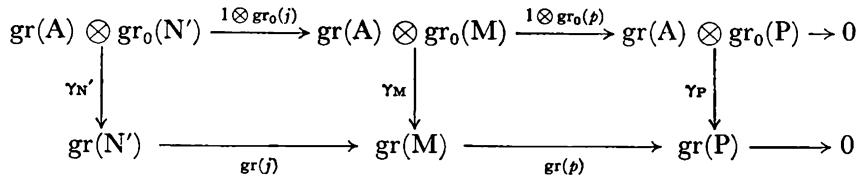
\includegraphics[keepaspectratio]{images/part002_c4775371.jpg}}

	下行是正合的（第 4 节，命题 2），而由第 4 节的命题 2 及 \(\mathrm{gr}_0(\mathbf{A})\) 是域这一事实，上行也正合。此外，\(\mathrm{gr}(j)\) 是单射（第 4 节，命题 2），因而 \(\mathrm{gr}_0(j)\) 是单射。对 \(j\) 应用论证的第一部分可知 \(\gamma_{\mathbf{N}'}\) 是双射；由于按假设 \(\gamma_{\mathbf{M}}\) 也是双射，故 \(\gamma_{\mathbf{P}}\) 是双射（第 I 章，§ 1，第 4 节，命题 2 的推论 2）。

推论。在命题 9 的假设下，若还假定 N 在 m-进滤过下是 Hausdorff 的，则 u 是单射。

这是因为 \(\operatorname{gr}(u)\) 是单射（定理 1 的推论 1）。

* 注。假设命题 9 的条件成立，并且下列条件之一也成立：

\begin{enumerate}
\def\labelenumi{(\arabic{enumi})}
\item
  m 是幂零的；
\item
  A 是 Noether 环且 P 是理想 Hausdorff 的（参见~§ 5，第 1 节）；
\end{enumerate}

则 P 是平坦 A-模。这由 \(\gamma_{P}\) 是双射及 § 5，第 2 节，定理 1 (iv) 得出，因为 A/m 是域。 *

\subsection{相伴分次模中元素族的提升}

设 A 为滤过交换环，\((\mathbf{A}_{n})_{n\in\mathbf{Z}}\) 为其滤过，C 为 \(A_{0}\) 的子环，满足 \(C\cap A_{1}=\{0\}\)。于是，\(\mathbf{A}_{0}\to\mathbf{A}_{0}/\mathbf{A}_{1}=\mathrm{gr}_{0}(\mathbf{A})\) 在 C 上的限制是单射，这使我们能够把 C 识别为 \(\mathrm{gr}_{0}(\mathbf{A})\) 的子模；类似情况下我们通常都这样做。若 \(A_{1}\neq A_{0}\)，且 K 是 \(A_{0}\) 的任意子域，则 \(K\cap A_{1}=\{0\}\)，因为 \(K\cap A_{1}\) 是 K 的不含 1 的理想；于是 K 可识别为 \(\mathrm{gr}_{0}(\mathbf{A})\) 的子域。

	命题 10. 设 A 为滤过交换环，\((\mathbf{A}_n)\) 为其滤过；假设存在子环 \(\mathbf{C}\)，它包含于 \(\mathbf{A}_0\)，使得 \(\mathbf{C} \cap \mathbf{A}_1 = \{0\}\)，并且将 \(\mathbf{C}\) 识别为 \(\operatorname{gr}_0(\mathbf{A})\) 的子环。设 \((x_i)_{1 \leqslant i \leqslant q}\) 是 \(\mathbf{A}\) 中的有限元素族；假设 \(x_i \in \mathbf{A}_{n_i}\) 对 \(1 \leqslant i \leqslant q\) 成立，并令 \(\xi_i\) 为 \(x_i\) 在 \(\operatorname{gr}_{n_i}(\mathbf{A})\) 中的类，对 \(1 \leqslant i \leqslant q\) 成立。

\begin{enumerate}
\def\labelenumi{(\roman{enumi})}
\item
	  若元素族 \((\xi_{i})\) 是 \(\operatorname{gr}(\mathbf{A})\) 中关于 \(\mathbf{C}\) 代数自由的元素族，则元素族 \((x_{i})\) 在 \(\mathbf{C}\) 上代数自由。
\item
  若 \(\mathbf{A}\) 上的滤过穷竭且离散，且 \((\xi_{i})\) 是 C-代数 \(\operatorname{gr}(\mathbf{A})\) 的生成系，则 \((x_{i})\) 是 C-代数 \(\mathbf{A}\) 的生成系。
\end{enumerate}

	令 \(\mathbf{A}'\) 为 \(\mathbf{C}[\mathbf{X}_1, \ldots, \mathbf{X}_q]\) 上的 \(\mathbf{C}\)-多项式代数；给 \(\mathbf{A}'\) 赋予分次 \((\mathbf{A}_n')\)，其类型为 \(\mathbf{Z}\)，其中 \(\mathbf{A}_n'\) 是单项式 \(\mathbf{X}_1^{s(1)} \ldots \mathbf{X}_q^{s(q)}\) 的 C-线性组合所成的集合，满足 \(\sum_{i=1}^{q} n_i s(i) = n\)。令 \(u\) 为同态 \(f \mapsto f(x_1, \ldots, x_q)\)，从 C-代数 \(\mathbf{A}'\) 到 C-代数 \(\mathbf{A}\)；按定义，\(u(\mathbf{A}_n') \subset \mathbf{A}_n\) 对所有 \(n \in \mathbf{Z}\) 成立，因而 \(u\) 与滤过相容（给 \(\mathbf{A}'\) 赋予与其分次环结构相伴的滤过环结构，参见~第 1 节，例 1）。因此，(i) 的假设意味着

\[
\operatorname{gr} (u): \mathrm{A} ^ {\prime} = \operatorname{gr} (\mathrm{A} ^ {\prime}) \rightarrow \operatorname{gr} (\mathrm{A})
\]

是单射；由于 A' 上的滤过穷竭且分离，可以应用第 8 节定理 1 的推论 1，故 u 是单射，这证明了 (i) 的结论。同样，关于 \((\xi_{i})\) 的假设 (ii) 意味着 gr(u) 是满射；由于 A 是离散的且其滤过穷竭，可以应用第 8 节定理 1 的推论 2，故 u 是满射，这证明了 (ii) 的结论。

	命题 11. 设 A 为完备 Hausdorff 滤过交换环，C 为 \(\mathbf{A}_0\) 的子环，满足 \(\mathbf{C} \cap \mathbf{A}_1 = 0\)，且 \((x_i)_{1 \leqslant i \leqslant q}\) 为 A 中的有限元素族，满足 \(x_i \in \mathbf{A}_{n_i}\)，其中 \(n_i > 0\) 对 \(1 \leqslant i \leqslant q\) 成立；令 \(\xi_i\) 为 \(x_i\) 在 \(\operatorname{gr}_{n_i}(\mathbf{A})\) 中的类，对 \(1 \leqslant i \leqslant q\) 成立。(i) 存在唯一的 C-同态 \(v\)，从形式幂级数代数 \(\mathbf{A}'' = \mathbf{C}[[\mathbf{X}_1, \ldots, \mathbf{X}_q]]\) 映到 A，并满足 \(v(\mathbf{X}_i) = x_i\) 对 \(1 \leqslant i \leqslant q\) 成立。

\begin{enumerate}
\def\labelenumi{(\roman{enumi})}
\setcounter{enumi}{1}
\item
  若族 \((\xi_{i})\) 在 \(\mathbf{C}\) 上代数自由，则同态 \(v\) 是单射。
\item
  若 \(\mathbf{A}\) 上的滤过穷竭，且族 \((\xi_{i})\) 是 C-代数 \(\operatorname{gr}(\mathbf{A})\) 的生成系，则同态 \(v\) 是满射。
\end{enumerate}

	由于 \(n_i \geqslant 1\) 对所有 \(i, \sum_{i=1}^{q} n_i s(i) \geqslant \sum_{i=1}^{q} s(i)\) 的情形，对每个单项式 \(X_1^{s(1)} \ldots X_q^{s(q)}\) 都有上述关系；另一方面，不等式 \(\sum_{i=1}^{q} n_i s(i) \leqslant r. \sum_{i=1}^{q} s(i)\) 在 \(r\) 为各 \(n_i\) 中最大的一个时成立。若 \(A_n''\) 表示由这样的形式幂级数所成的集合：其非零项 \(a_s X_1^{s(1)} \ldots X_q^{s(q)}\) 满足 \(\sum_{i=1}^{q} n_i s(i) \geqslant n\)，则由第 6 节命题 6 的推论可知，\(A''\) 在穷竭滤过 \((A_n'')\) 下是 Hausdorff 且完备的，并且

\[
\mathrm{A} ^ {\prime} = \mathrm{C} [ \mathrm{X} _ {1}, \dots , \mathrm{X} _ {q} ]
\]

在 A'' 中稠密；此外，证明命题 10 时定义的同态 u 在 A' 上连续，并且由于 A 是 Hausdorff 且完备的，可以唯一延拓为连续同态 v: A''→A（《一般拓扑学》，第 III 章，§ 3，第 3 节，命题 5），这证明了 (i)；又有 gr(A'') = gr(A') 且 gr(v) = gr(u)；根据 A 的假设，(ii) 和 (iii) 分别由第 8 节定理 1 的推论 1 和 2 得出。

命题的 (ii)（分别 (iii)）的结论有时表述为：族 \((x_{i})\) 在 C 上形式自由（分别是 A 的形式生成系）。

命题 12. 设 A 为滤过环，E 为滤过 A-模，\((\mathbf{A}_{n})\) 和 \((\mathbf{E}_{n})\) 分别是 A 和 E 上的滤过。假设 A 完备且滤过 \((\mathbf{E}_{n})\) 穷竭并分离。设 \((x_{i})_{i\in\mathbf{I}}\) 是 E 中的有限元素族，并对 \(i\in I\) 令 \(n(i)\) 为满足 \(x_{i}\in\mathbf{E}_{n(i)}\) 的整数；最后令 \(\xi_{i}\) 为 \(x_{i}\) 在 \(\mathrm{gr}_{n(i)}(\mathbf{E})\) 中的类。则若 \((\xi_{i})\) 是 gr(A)-模 gr(E) 的生成系，\((x_{i})\) 是 A-模 E 的生成系。

	在 A-模 \(\mathbf{L} = \mathbf{A}_s^{\mathbf{I}}\) 中，令 \(\mathbf{L}_n\) 表示由 \((a_i)\) 所成的集合，其中 \(a_i \in \mathbf{A}_{n - n(i)}\) 对所有 \(i \in \mathbf{I}\) 成立；若 \(p\) 和 \(q\) 分别是 \(n(i)\) 中最小和最大的，则 \(\mathbf{A}_{n - q}^{\mathbf{I}} \supset \mathbf{L}_n \supset \mathbf{A}_{n - p}^{\mathbf{I}}\)，并且由 \(\mathbf{L}\) 上的定义 \((\mathbf{L}_n)\) 所确定的拓扑就是乘积拓扑；因此 \(\mathbf{L}\) 是完备滤过 A-模。由于 \(\mathbf{L}\) 是自由模，存在一个

A-线性映射 \(u: \mathbf{L} \to \mathbf{E}\)，满足 \(u((a_i)) = \sum_{i \in \mathbf{I}} a_i x_i\)，且它显然与滤过相容；我们必须证明 \(u\) 是满射，而根据第 8 节定理 1 的推论 2，为此只需证明

\[
\operatorname{gr} (u): \operatorname{gr} (\mathbf {L}) \rightarrow \operatorname{gr} (\mathbf {E})
\]

	是满射；或者等价地，对所有 \(x \in \mathbf{E}_n\)，存在一个族 \((a_i)\)，使 \(a_i \in \mathbf{A}_{n-n(i)}\) 对所有 \(i \in I\) 成立，且 \(x \equiv \sum_{i \in I} a_i x_i \pmod{\mathbf{E}_{n+1}}\)。令 \(\xi\) 为 \(x\) 在 \(\mathrm{gr}_n(\mathbf{E})\) 中的类；由于 \(\xi_i\) 生成 \(\mathrm{gr}(\mathbf{A})\)-模 \(\mathrm{gr}(\mathbf{E})\)，存在 \(\alpha_i \in \mathrm{gr}(\mathbf{A})\)，使得 \(\xi = \sum_{i \in I} \alpha_i \xi_i\)，并且假设 \(\alpha_i \in \mathrm{gr}_{n-n(i)}(\mathbf{A})\)；必要时可将 \(\alpha_i\) 替换为其 \(n - n(i)\) 次齐次分量。于是 \(\alpha_i\) 是某个 \(a_i \in \mathbf{A}_{n-n(i)}\) 的像，族 \((a_i)\) 具有所要求的性质。

推论 1. 设 A 为完备滤过环，E 为滤过 A-模，且其滤过穷竭并分离。若 gr(E) 是有限生成的（分别为 Noether 的）gr(A)-模，则 E 是有限生成的（分别为 Noether 的）A-模。

若 \(\mathrm{gr}(\mathrm{E})\) 有限生成，则存在有限齐次生成系，由命题 12 可知 E 有限生成。现在假设 \(\mathrm{gr}(\mathrm{E})\) 是 Noether 的，并设 F 为 E 的子模；由 E 上的滤过在 F 上诱导的滤过穷竭且分离，而 \(\mathrm{gr}(\mathrm{F})\) 可识别为 gr(E) 的一个 gr(A)-子模（第 4 节，命题 2），故由假设它有限生成；于是 F 是有限生成 A-模，从而 E 是 Noether 模。

推论 2. 设 A 为完备 Hausdorff 滤过环，且其滤过穷竭。若 gr(A) 是左 Noether 环，则 A 也是左 Noether 环。

只需将推论 1 应用于 \(\mathbf{E} = \mathbf{A}_s\) 即可。

推论 3. 设 A 为完备滤过环，\((\mathbf{A}_{n})\) 为其滤过，E 为 Hausdorff 滤过 A-模，\((\mathbf{E}_{n})\) 为其滤过，F 为 E 的有限生成子模；假设 \(A_{0} = A\) 且 \(E_{0} = E\)。

\begin{enumerate}
\def\labelenumi{(\roman{enumi})}
\item
  若对所有 \(k \geqslant 0\) 都有 \(\mathbf{E}_k = \mathbf{E}_{k+1} + \mathbf{A}_k\mathbf{F}\)，则 \(\mathbf{F} = \mathbf{E}\)。
\item
  若进一步假设 \(\mathbf{E}\) 上的滤过由 \(\mathbf{A}\) 上的滤过导出（第 1 节，例 2），则关系 \(\mathbf{E} = \mathbf{E}_1 + \mathbf{F}\) 蕴含 \(\mathbf{F} = \mathbf{E}\)。
\end{enumerate}

	令 \(\xi_{i}(1\leqslant i\leqslant n)\) 为 \(\mathbf{E}_1\) 模下 \(\mathbf{F}\) 的一个有限生成系的类。由给定假设，对所有 \(k\geqslant 0\)，\(\mathrm{gr}_k(\mathrm{E})\) 的每个元素

	都可写成 \(\sum_{i=1}^{\infty} \alpha_i \xi_i\) 的形式，其中 \(\alpha_i \in \mathrm{gr}(A)\)；因此 \(\xi_i\) 生成 \(\mathrm{gr}(A)\)-模 \(\mathrm{gr}(E)\)，由命题 12 得到 (i)。若 \(E\) 上的滤过由 \(A\) 上的滤过导出，则关系 \(E = E_1 + F\) 蕴含

\[
\begin{array}{r} \mathbf {E} _ {k} = \mathbf {A} _ {k} \mathbf {E} = \mathbf {A} _ {k} \mathbf {E} _ {1} + \mathbf {A} _ {k} \mathbf {F} = \mathbf {A} _ {k} \mathbf {A} _ {1} \mathbf {E} + \mathbf {A} _ {k} \mathbf {F} \subset \mathbf {A} _ {k + 1} \mathbf {E} + \mathbf {A} _ {k} \mathbf {F} \\ = \mathbf {E} _ {k + 1} + \mathbf {A} _ {k} \mathbf {F} \subset \mathbf {E} _ {k}, \end{array}
\]

从而得到 (ii)。

命题 13. 设 A 为环，m 为包含在 A 的 Jacobson 根中的 A 的双边理想，E 为 A-模。给 A 和 E 赋予 m-进滤过（第 1 节，例 3）。假设下列条件之一成立：

\begin{enumerate}
\def\labelenumi{(\alph{enumi})}
\item
  E 是有限生成 A-模且 A 是 Hausdorff 的；
\item
  m 是幂零的。
\end{enumerate}

E 是自由 A-模的充要条件是：E/mE 是自由 (A/m)-模，且 E 满足性质 (GR)（第 8 节）。

	若 E 是自由 A-模，且 \((e_{\lambda})\) 是 E 的一组基，则 \(m^{k}E\) 是 E 中各子模 \(m^{k}e_{\lambda}\) 的直和，对所有 \(k \geqslant 0\) 成立（《代数》，第 II 章，§3，第 7 节，注）；于是 \(m^{k}E/m^{k+1}E\) 可识别为各 \(m^{k}e_{\lambda}/m^{k+1}e_{\lambda}\) 的直和（《代数》，第 II 章，§1，第 6 节，命题 7）。我们首先（当 k = 0 时）得到，各 \(1 \otimes e_{\lambda}\) 是各 \(e_{\lambda}\) 的类，并且它们位于 E/mE = (A/m) \(\otimes_{A} E\) 中，构成 (A/m)-模 E/mE 的一组基，因为典范映射

\[
\left(\mathfrak {m} ^ {k} / \mathfrak {m} ^ {k + 1}\right) \otimes_ {\mathbf {A}} (\mathrm{E} / \mathfrak {m} \mathrm{E}) \rightarrow \mathfrak {m} ^ {k} \mathrm{E} / \mathfrak {m} ^ {k + 1} \mathrm{E}
\]

	对于所有 \(k \geqslant 0\) 都是双射；因此 \(\gamma_{\mathbf{E}}\) 是双射。注意，证明的这一部分既未用到条件 (a)，也未用到条件 (b)。

	反之，设命题条件成立，并令 \((x_{\iota})_{\iota \in I}\) 是 E 中一族元素，其模 mE 的类构成 (A/m)-模 E/mE 的一组基；令 L 为自由 A-模 \(\mathrm{A}_s^{(I)}\)，\((f_{\iota})_{\iota \in I}\) 为其典范基，并令 \(u: \mathbf{L} \to \mathbf{E}\) 为满足 \(u(f_{\iota}) = x_{\iota}\)（对所有 \(\iota \in I\)）的 A-线性映射。命题的假设已蕴含 \(u\) 为满射（第 II 章，§3，第 2 节，命题 4 的推论 1），所以只需证明 \(u\) 为单射。现在，条件 (a) 和 (b) 中的每一个都蕴含 A 是 Hausdorff 的，因而带 m-进滤过的 L 也具有此性质，因为 \(\mathfrak{m}^k\mathbf{L} = (\mathfrak{m}^k)^{(I)}\)（《代数》，第 II 章，§3，第 7 节，注），且 \(\operatorname{gr}(\mathbf{L})\) 可根据证明的第一部分识别为 \(\operatorname{gr}(\mathbf{A}) \otimes_{\mathbf{A} / \mathfrak{m}} (\mathbf{L} / \mathfrak{m}\mathbf{L})\)；同态 \(u\) 与滤过相容，并且可以写成 \(\operatorname{gr}(u) = \gamma_{\mathbb{E}} \circ v\)，其中 \(v\) 是把 \(\operatorname{gr}(\mathbf{L})\) 双射到

\[
\operatorname{gr} (\mathbf {A}) \otimes_ {\mathbf {A} / \mathfrak {m}} (\mathbf {E} / \mathfrak {m} \mathbf {E})
\]

	将 \(f_{t}\) 模 mM 的类映到 \(1 \otimes \bar{x}_{t}\)，其中 \(\bar{x}_{t}\) 是 \(x_{t}\) 模 mE 的类。于是该假设蕴含 \(\operatorname{gr}(u)\) 是单射，结论由第 8 节定理 1 的推论 1 得出。

\subsection{应用：Noether 环的例子}

		引理 1. 设 A 为 Z 型分次环，其分次（\(A_{n}\)）满足 \(A_{n} = 0\) 对所有 n \textless{} 0，或者 \(A_{n} = 0\) 对所有 n \textgreater{} 0。设 M 为 Z 型分次 A-模。M 是 Noether A-模的充要条件是 M 的每个分次子模都是有限生成的。

	由于 \(n \mapsto -n\) 是群 \(\mathbf{Z}\) 的自同构，我们可以只考虑 \(A_n = 0\) 对所有 \(n > 0\) 的情形。令 \(A'\) 和 \(M'\) 分别表示带有与各自分次相伴的滤过的环 \(A\) 和模 \(M\)（第 1 节，例 1），这些滤过是穷竭且分离的；关于 \(A\) 的假设蕴含 \(A'\) 是离散的，因而是完备的。若 \(E\) 是 \(M\) 的一个 A-子模，则所得到的滤过 \(A'\)-模 \(E'\)（在 \(E\) 上赋予诱导滤过）是 Hausdorff 的，且其滤过是穷竭的；此外，\(\text{gr}(E')\) 可识别为 \(M = \text{gr}(M')\) 的一个分次 A-子模，因而由假设有限生成。结论于是由第 9 节命题 12 的推论 1 得出。

	定理 2. 设 A 为 N 型分次环，M 为 N 型分次 A-模，\((\mathbf{A}_{n})\) 和 \((\mathbf{M}_{n})\) 分别为它们的分次。假设存在元素 \(a \in A_{1}\)，使得 \(A_{n} = A_{0}a^{n}\) 且 \(M_{n} = a^{n}M_{0}\) 对所有 n \textgreater{} 0 成立。那么，如果 \(M_{0}\) 是 Noether \(A_{0}\)-模，M 就是 Noether A-模。

	由引理 1，只需证明 M 的每个分次子模 N 都是有限生成的。对所有 \(r \geqslant 0\)，令 \(\mathbf{N}_r = \mathbf{N} \cap \mathbf{M}_r\)，并令 \(\mathbf{L}_r\) 为 \(m \in \mathbf{M}_0\) 中满足 \(a^r m \in \mathbf{N}_r\) 的元素所成的集合。由于

\[
a ^ {r} \mathrm{A} _ {0} \subset \mathrm{A} _ {r} = \mathrm{A} _ {0} a ^ {r}, \quad a ^ {r} \mathrm{A} _ {0} \mathrm{L} _ {r} \subset \mathrm{A} _ {0} a ^ {r} \mathrm{L} _ {r} \subset \mathrm{A} _ {0} \mathrm{N} _ {r} \subset \mathrm{N} _ {r}
\]

	所以 \(L_{r}\) 是 \(A_{0}\)-模 \(M_{0}\) 的子模；此外，

\[
a \mathrm{N} _ {r} \subset \mathrm{N} \cap a \mathrm{M} _ {r} = \mathrm{N} \cap \mathrm{M} _ {r + 1} = \mathrm{N} _ {r + 1}
\]

	所以序列 \((\mathbf{L}_{r})_{r\geqslant0}\) 递增。假设蕴含存在整数 \(n\geqslant0\)，使 \(L_{r}=L_{n}\) 对 \(r\geqslant n\) 成立。对每个 \(r\leqslant n\)，令 \((m_{r,s})_{1\leqslant s\leqslant k_{r}}\) 为 \(A_{0}\)-模 \(L_{r}\) 的一组生成元。我们将证明，元素 \(a^{r}m_{r,s}\) 对 \(1\leqslant s\leqslant k_{r}, 0\leqslant r\leqslant n\) 构成 A-模 N 的一组生成元。由于 \(M_{r}=a^{r}M_{0}\) 对所有 r 成立，\(N_{r}=a^{r}L_{r}\) 对所有 r 成立，这是按 \(L_{r}\) 的定义。于是，当 \(r\leqslant n\) 时，

\[
\mathbf {N} _ {r} = a ^ {r} \mathbf {L} _ {r} = \sum_ {s = 1} ^ {k _ {r}} a ^ {r} \mathbf {A} _ {0} m _ {r, s} \subset \sum_ {s = 1} ^ {k _ {r}} \mathbf {A} _ {0} a ^ {r} m _ {r s},
\]

并且，对于 \(r > n\)，

\[
\mathrm{N} _ {r} = a ^ {r} \mathrm{L} _ {n} = \sum_ {s = 1} ^ {k _ {n}} a ^ {r} \mathrm{A} _ {0} m _ {n, s} \subset \sum_ {s = 1} ^ {k _ {n}} \mathrm{A} _ {0} a ^ {r} m _ {n, s} \subset \sum_ {s = 1} ^ {k _ {n}} \mathrm{A} _ {0} a ^ {r - n}. (a ^ {n} m _ {n, s})
\]

	这就完成了证明（参见~习题 10）。

	推论 1（Hilbert 定理）。对于每个交换 Noether 环 C，多项式环 C{[}X{]} 都是 Noether 环（参见~习题 10）。

	推论 2. 对于每个交换 Noether 环 C 以及每个整数 n \textgreater{} 0，多项式环 C{[}X₁, \ldots, Xₙ{]} 都是 Noether 环。

	这是由推论 1 对 n 作归纳得到的。

	推论 3. 若 C 是交换 Noether 环，则每个有限生成的交换 C-代数都是 Noether 环。

	这样的代数同构于多项式代数 \(\mathbf{C}[\mathbf{X}_1,\ldots ,\mathbf{X}_n]\) 的一个商（第 1 节，第 1 节）。

	推论 4. 设 A 为 N 型分次交换环，\((\mathbf{A}_{n})\) 为其分次。A 为 Noether 环的充要条件是 \(A_{0}\) 为 Noether 环且 A 是有限生成的 \(A_{0}\)-代数。

	由推论 3，所述条件是充分的。反之，设 A 是 Noether 环；\(m = \sum_{n \geqslant 1} A_n\) 是 A 的一个理想，因而有限生成；于是 A 是有限生成的 \(A_0\)-代数（第 1 节，第 2 节，命题 1 的推论）；另一方面，\(A_0\) 同构于 A/m，是 Noether 环。

	推论 5. 设 A 为交换环，m 为 A 的理想，且 A/m 是 Noether 环，m/m² 是有限生成的 (A/m)-模，并且 A 在 m-进拓扑下 Hausdorff 且完备。那么 gr(A) 和 A 都是 Noether 环。

	\(\operatorname{gr}(\mathbf{A})\) 是由 \((\mathbf{A} / \mathfrak{m})\)-模 \(\mathfrak{m} / \mathfrak{m}^2\) 生成的（第 3 节，例 3），因而由推论 3，环 gr(A) 是 Noether 环。由此得到 A 本身是 Noether 环（第 9 节，命题 12 的推论 2）。

	推论 6. 对于每个交换 Noether 环 C 以及每个整数 n \textgreater{} 0，形式幂级数环 C{[}{[}X₁, \ldots, Xₙ{]}{]} 都是 Noether 环。

	这是由推论 5 以及第 6 节命题 6 的推论得到的，因为若 m 是 A = C{[}{[}X₁, \ldots, Xₙ{]}{]} 中由没有常数项的形式幂级数构成的理想，则 A/m 同构于 C，而 m/m² 同构于 C-模 Cⁿ。

\textbf{注}\par

\begin{enumerate}
\def\labelenumi{(\arabic{enumi})}
\tightlist
\item
	  推论 2、3 和 6 尤其适用于 C 为交换域的情形。
\end{enumerate}

	* (2) 设 g 为交换 Noether 环 C 上的李代数，并假设 g 是有限生成的 C-模。给 g 的包络代数 U 赋予第 3 节例 4 中定义的递增滤过 \((\mathbf{U}_{n})\)。在相应拓扑下，U 是离散的，因而 Hausdorff 且完备；相伴的分次环 gr(U) 是有限生成的 C-代数，因为它是对称代数 S(g) 的一个商，因而 gr(U) 是 Noether 环（推论 3），于是我们得到 U 是左、右 Noether 环（第 9 节，命题 12 的推论 2）。 *

\subsection{完备的 m-进环与逆极限}

	我们在第 6 节已经看到，若 A 为交换环，m 为 A 的理想，且 A 在 m-进拓扑下 Hausdorff 且完备，则拓扑环 A 可典范识别为离散环 \(A_{i} = A/m^{i+1} (i \in \mathbf{N})\) 关于典范映射所成的逆极限

\[
h _ {i j} \colon \mathrm{A} / \mathfrak {m} ^ {j + 1} \rightarrow \mathrm{A} / \mathfrak {m} ^ {i + 1} \quad (i \leqslant j);
\]

	注意，\(h_{ij}\) 是满射，并且若 \(n_{ij}\) 是其核，则

\[
\mathfrak {n} _ {i j} = \mathfrak {m} ^ {i + 1} / \mathfrak {m} ^ {j + 1} = (\mathfrak {m} / \mathfrak {m} ^ {j + 1}) ^ {i + 1} = (\mathfrak {n} _ {0 j}) ^ {i + 1};
\]

	特别地，\((\mathfrak{n}_{0j})^{j + 1} = 0\)。反之：

	命题 14. 设 \((\mathbf{A}_i, h_{ij})\) 是离散交换环的一个逆系统，其指标集为 \(\mathbf{N}\)，并设 \((\mathbf{M}_i, u_{ij})\) 是环逆系统 \((\mathbf{A}_i, h_{ij})\) 上模的一个逆系统。令 \(\mathfrak{n}_j\) 表示 \(h_{0j} \colon \mathbf{A}_j \to \mathbf{A}_0\) 的核，并置 \(\mathbf{A} = \varprojlim \mathbf{A}_i\)、\(\mathbf{M} = \lim \mathbf{M}_i\)。假设

\begin{enumerate}
\def\labelenumi{(\alph{enumi})}
\item
	  对所有 \(i \in \mathbf{N}\)，\(h_{i1}\) 是 \(A_i\) 上的恒等映射，并且对于 \(i \leqslant j\)，\(h_{i1}\) 和 \(u_{i1}\) 都是满射；
\item
	  对 \(i \leqslant j\)，\(h_{ij}\) 和 \(u_{ij}\) 的核分别为 \(\mathfrak{n}_j^{i+1}\) 和 \(\mathfrak{n}_j^{i+1}\mathrm{M}_j\)。
\end{enumerate}

	则：

\begin{enumerate}
\def\labelenumi{(\roman{enumi})}
\item
	  A 是完备 Hausdorff 拓扑环，M 是完备 Hausdorff 拓扑 A-模，并且典范映射 \(h_{i}: A \to A_{t}, u_{i}: M \to M_{i}\) 是满射。
\item
	  若 \(M_{0}\) 是有限生成的 \(A_{0}\)-模，则 M 是有限生成的 A-模；

	  确切地说，M 的每个有限子集 S，只要 \(u_{0}(S)\) 生成 \(M_{0}\)，就是 M 的一组生成元。
\end{enumerate}

	(i) 中的断言由《一般拓扑学》第 II 章 § 3 第 5 节命题 10 的推论和定理 1 的推论 1 得出。

	对所有 \(i \in \mathbf{N}\)，记 \(\mathfrak{m}_{i+1} = \operatorname{Ker}(h_i)\)、\(\mathbf{N}_{i+1} = \operatorname{Ker}(u_i)\)；则

\[
\mathfrak {m} _ {i + 1} = \varprojlim_ {k \geqslant 0} h _ {i, i + k} ^ {- 1} (0) = \varprojlim_ {k} \mathfrak {n} _ {i + 1} ^ {i + k}
\]

	并且 \(\mathbf{N}_{i + 1} = \lim_{k\to \infty}\mathfrak{n}_{i + k}^{i + 1}\mathbf{M}_{i + k}\)；由于 \(h_{i + k}\) 和 \(u_{i + k}\) 是满射，

\[
h _ {i + k} \left(\mathfrak {m} _ {i + 1}\right) = \mathfrak {n} _ {i + k} ^ {i + 1}, \quad u _ {i + k} \left(\mathrm{N} _ {i + 1}\right) = \mathfrak {n} _ {i + k} ^ {i + 1} \mathrm{M} _ {i + k}.\tag{16}
\]

	我们证明 \(\mathfrak{m}_i\mathrm{N}_j\subset \mathrm{N}_{i + j}\) 当 \(i\geqslant 1\)、\(j\geqslant 1\) 时成立，这等价于证明 \(u_{i + j - 1}(\mathfrak{m}_i\mathrm{N}_j) = 0\)；现在

\[
u _ {i + j - 1} (m _ {i} \mathrm{N} _ {j}) = h _ {i + j - 1} (m _ {i}) u _ {i + j - 1} (\mathrm{N} _ {j})
\]

	这等于 \(\mathfrak{n}_{i+j-1}^{i}(\mathfrak{n}_{i+j-1}^{j}\mathrm{M}_{i+j-1}) = 0\)，因为对所有 \(k \geqslant 0\)，\(\mathfrak{n}_k^{k+1}\) 是 \(h_{kk}\) 的核，且等于 0。类似地可见 \(\mathfrak{m}_i\mathfrak{m}_j \subset \mathfrak{m}_{i+j}\)。若对 \(i \leqslant 0\) 置 \(\mathfrak{m}_i = \mathrm{A}\) 且 \(\mathrm{N}_i = \mathrm{M}\)，则 \((\mathfrak{m}_i)_{i \in \mathbf{Z}}\) 是 \(\mathrm{A}\) 的滤过，\((\mathrm{N}_i)_{i \in \mathbf{Z}}\) 是 \(\mathrm{M}\) 的滤过，并且与 \(\mathrm{A}\) 上的滤过相容；\(\mathrm{A}\) 和 \(\mathrm{M}\) 上的拓扑显然就是由这些滤过定义的拓扑。于是，令 \(\mathfrak{a}\) 为 \(\mathrm{A}\) 的理想，使得 \(h_1(a) = \mathfrak{n}_1\)，并令 \(\mathrm{M}'\) 为 \(\mathrm{M}\) 中由 \(\mathrm{S}\) 生成的子模；我们将证明

\[
\mathrm{N} _ {i} = \mathfrak {a} ^ {i} \mathrm{M} ^ {\prime} + \mathrm{N} _ {i + 1} \quad \text { for } \quad i \geqslant 0.\tag{17}
\]

	记 \(a_i = h_i(a), M'_i = u_i(M')\)；只需证明

\[
u _ {i} \left(\mathrm{N} _ {i}\right) = a _ {i} ^ {t} \mathrm{M} _ {i} ^ {\prime}.
\]

	当 \(i = 0\) 时这成立，因为由假设 \(\mathbf{N}_0 = \mathbf{M}\) 且 \(\mathbf{M}_0' = \mathbf{M}_0\)。若 \(i \geqslant 1\)，则由 (16) 有 \(u_i(\mathbf{N}_i) = \mathfrak{n}_i^i\mathbf{M}_i\)。由于 \(h_{1i}\) 是满射且 \(h_{0i} = h_{01} \circ h_{1i}\)，\(h_{1i}\) 把核 \(\mathfrak{n}_i\)（即 \(h_{0i}\) 的核）映到核 \(\mathfrak{n}_1\)（即 \(h_{01}\) 的核），并且 \(\mathfrak{n}_t = \overline{h}_{1i}^{-1}(\mathfrak{n}_1)\)；于是

\[
h _ {1 i} (a _ {i}) = h _ {1} (a) = n _ {1} = h _ {1 i} (n _ {i})
\]

	又由于 \(h_{1i}\) 的核为 \(n_i^2\)，有 \(n_i \subset a_i + n_i^2\) 且 \(a_i \subset n_i\)，从而 \(n_i = a_i + n_i^2\)。此外，\(u_{0i}(M_i') = u_0(M') = M_0 = u_{0i}(M_i)\)，又由于 \(\text{Ker}(u_{0i}) = n_iM_i\)，有 \(M_t = M_t' + n_iM_t\)；从而

\[
n _ {i} ^ {t} \mathbf {M} _ {i} = (a _ {i} + n _ {i} ^ {2}) ^ {t} (\mathbf {M} _ {i} ^ {\prime} + n _ {i} \mathbf {M} _ {i}).
\]

	现在，\(\mathfrak{a}_i^k\mathfrak{n}_i^{i + 1 - k}\subset \mathfrak{n}_i^{i + 1} = 0\) 对 \(0\leqslant k\leqslant i\) 成立；于是显然 \(u_{i}(\mathbf{N}_{i}) = \mathfrak{n}_{i}\mathbf{M}_{i} = \mathfrak{a}_{i}^{i}\mathbf{M}_{t}^{\prime}\)，这就证明了 (17)。

	此外，\(m_1 = h_1(n_1)\)，从而 \(a \subset m_1\)，因此 \(a^t \subset m_1^t \subset m_i\)，从而

	\(N_{i} \subset m_{i}M' + N_{i+1}\)；另一方面显然 \(m_{i}M \subset N_{i}\)，从而 \(N_{i} = m_{i}M' + N_{i+1}\) 对所有 \(i \geqslant 0\) 成立；于是由第 9 节命题 12 的推论 3 得到 \(M' = M\)，证明完毕。

	推论 1. 在命题 14 的记号和假设下，进一步假设 \(\mathbf{M}_0\) 是有限生成的 \(\mathbf{A}_0\)-模，且理想 \(\mathfrak{n}_1\) 是 \(\mathbf{A}_1\) 的有限生成理想。令 \(\mathfrak{m}_1\) 为 \(h_0\) 的核；于是 \(\mathbf{A}\) 和 \(\mathbf{M}\) 上的拓扑分别是这个环和这个模上的 \(\mathfrak{m}_1\)-进拓扑；确切地说，对所有 \(i \geqslant 0\)，\(h_i\) 和 \(u_i\) 的核分别为 \(\mathfrak{m}_1^{i+1}\) 和 \(\mathfrak{m}_1^{i+1}\mathbf{M}\)；此外，\(\mathfrak{m}_1/\mathfrak{m}_1^2\) 是有限生成的 A-模。

	我们沿用命题 14 证明中的记号；这里的假设允许我们假定理想 a 是有限生成的。令 \(i \geqslant 0\) 为任意整数；对所有 \(j \geqslant 0\)，由 (17) 有 \(\mathbf{N}_{i+j} = \mathfrak{a}^j (\mathfrak{a}^i\mathbf{M}) + \mathbf{N}_{i+j+1} \subset \mathfrak{m}_j(\mathfrak{a}^i\mathbf{M}) + \mathbf{N}_{i+j+1}\)；反之，\(\mathfrak{m}_j(\mathfrak{a}^i\mathbf{M}) \subset \mathfrak{m}_j\mathfrak{m}_i\mathbf{M} \subset \mathfrak{m}_{i+j}\mathbf{M} \subset \mathbf{N}_{i+j}\)，从而

\[
\mathbf {N} _ {i + j} = \mathfrak {m} _ {j} (\mathfrak {a} ^ {i} \mathbf {M}) + \mathbf {N} _ {i + j + 1}.
\]

	由于 a 和 M 是有限生成的 A-模，\(a^{i}M\) 也是有限生成的 A-模。将第 9 节的命题 12 的推论 3 应用于模 \(N_{i}\) 及其滤过 \((\mathrm{N}_{ij})_{j\in\mathbf{Z}}\)，其中滤过定义为：\(N_{ij}=N_{i}\) 当 j\textless0 时；\(N_{ij}=N_{i+j}\) 当 \(j\geqslant0\) 时，由此得到 \(N_{i}=a^{i}M\)，从而 \(N_{i}\subset m_{1}^{i}M\)。但同样有 \(m_{1}^{i}M\subset m_{i}M\subset N_{i}\)，所以 \(N_{i}=m_{1}^{i}M\)。将此应用于 \(M_{i}=A_{i}\)、\(u_{ij}=h_{ij}\) 的情形，得到 \(m_{i}=m_{1}^{i}\)。此外，根据 (17)，\(m_{1}=a+m_{1}^{2}\)，这就证明了推论的最后一个断言。

	推论 2. 在推论 1 的假设下，A 为 Noether 环的充要条件是 \(A_{0}\) 为 Noether 环。

	必要性是因为 \(A_{0}\) 同构于 A 的一个商；充分性由第 10 节定理 2 的推论 5 得出。

\subsection{滤过模的 Hausdorff 完备化}

令 G 为一个滤过群，其滤过 \((\mathbf{G}_{n})\) 由 G 的正规子群组成；我们已经在第 6 节回顾过，拓扑群 G 的 Hausdorff 完备化 \(\hat{G}\) 可典范地识别为离散群的逆极限 \(\lim_{\substack{\mathbf{G}/\mathbf{G}_{n}\\ }} \overleftarrow{\mathbf{G}}\)，其中离散群为 \(G/G_{n}\)；典范同态 \(i: G \to \hat{G}\) 的像是与 G 相关的 Hausdorff 群（在 \(\hat{G}\) 中处处稠密），其核是闭包 \(\bigcap G_{n}\)，即 G 中 \(\{0\}\) 的闭包。G 的子群的 Hausdorff 完备化 \(\hat{G}_{n}\)（子群为 \(G_{n}\)）可识别为 \(i(\mathbf{G}_{n})\) 在 \(\hat{G}\) 中的闭包（《一般拓扑学》，第二章 §3，第 9 节，命题 18 的推论 1），并且由于 \(G_{n}\) 在 G 中是闭的，


\[
\mathbf {G} _ {n} = \stackrel {- 1} {i} (\hat {\mathbf {G}} _ {n}) = \stackrel {- 1} {i} (\hat {\mathbf {G}} _ {n} \cap i (\mathbf {G})).\tag{18}
\]

此外，\(\hat{G}_n\) 构成 \(\hat{G}\) 中 0 的邻域基本系（《一般拓扑学》，第三章 §3，第 4 节，命题 7），因而是 \(\hat{\mathbf{G}}\) 的正规开子群（《一般拓扑学》，第三章 § 2，第 3 节，命题 8）；\(\hat{\mathbf{G}}\) 上的拓扑由滤过 \((\hat{\mathbf{G}}_n)\) 定义，按定义总是分离的。由于 \(i(\mathbf{G})\) 在 \(\hat{\mathbf{G}}\) 中稠密且 \(\hat{\mathbf{G}}_n\) 是开集，

\[
\hat {\mathbf {G}} = i (\mathbf {G}). \hat {\mathbf {G}} _ {n}\tag{19}
\]

同样有

\[
\hat {\mathbf {G}} _ {n - 1} = i \left(\mathbf {G} _ {n - 1}\right). \hat {\mathbf {G}} _ {n}.\tag{20}
\]

由 (18) 和 (19) 可得，滤过 \((\hat{G}_n)\) 是穷竭的，当且仅当滤过 \((G_n)\) 是穷竭的。

第二同构定理（《代数》，第一章 § 6，第 13 节，定理 6 (d)）以及等式 (18)、(19) 和 (20) 表明，典范同态

\[
\mathrm{G} _ {n - 1} / \mathrm{G} _ {n} \rightarrow \hat {\mathrm{G}} _ {n - 1} / \hat {\mathrm{G}} _ {n}, \quad \mathrm{G} / \mathrm{G} _ {n} \rightarrow \hat {\mathrm{G}} / \hat {\mathrm{G}} _ {n},\tag{21}
\]

都是双射，因而典范同态

\[
\operatorname{gr} (\mathbf {G}) \rightarrow \operatorname{gr} (\hat {\mathbf {G}}).\tag{22}
\]

现在设 A 是一个滤过环，E 是一个滤过 A-模，而 \((\mathbf{A}_{n})\) 和 \((\mathbf{E}_{n})\) 分别是 A 和 E 的滤过；我们假设这些滤过是穷竭的，从而相应的拓扑使 A 成为拓扑环、E 成为拓扑 A-模（第 5 节，命题 3）。于是我们已经定义了（《一般拓扑学》，第三章 § 6，第 5、6 节）拓扑环 \(\hat{A}\) 和拓扑模 \(\hat{E}\)，后者是拓扑 \(\hat{A}\)-模。若 \(i: A \to \hat{A}\) 是典范同态，则 \(i(\mathbf{A}_{m})i(\mathbf{A}_{n}) \subset i(\mathbf{A}_{m+n})\)，因此由 \(\hat{A}\) 中乘法的连续性，

\[
\hat {\mathrm{A}} _ {m} \hat {\mathrm{A}} _ {n} \subset \hat {\mathrm{A}} _ {m + n}\tag{23}
\]

因为 \(\hat{\mathbf{A}}_n\) 是 \(i(\mathbf{A}_n)\) 在 \(\hat{\mathbf{A}}\) 中的闭包。类似地可证明

\[
\hat {\mathrm{A}} _ {m} \hat {\mathrm{E}} _ {n} \subset \hat {\mathrm{E}} _ {m + n};\tag{24}
\]

换言之：

命题 15. 设 A 是一个滤过环，E 是一个滤过 A-模，A 和 E 的相应滤过 \((\mathbf{A}_{n})\)、\((\mathbf{E}_{n})\) 是穷竭的。那么 \((\hat{\mathbf{A}}_{n})\) 是一个与 \(\hat{A}\) 的环结构相容的滤过，而 \((\hat{\mathbf{E}}_{n})\) 是一个与 \(\hat{E}\) 上的模结构相容的滤过，该模结构来自滤过环 \(\hat{A}\)；此外，这些滤过是穷竭的，并分别定义 \(\hat{A}\) 和 \(\hat{E}\) 上的拓扑。最后，分次 Z-模的典范映射 \(\mathrm{gr}(\mathbf{A}) \to \mathrm{gr}(\hat{\mathbf{A}})\) 和 \(\mathrm{gr}(\mathrm{E}) \to \mathrm{gr}(\hat{\mathrm{E}})\) 分别是分次环同构和分次 gr(A)-模同构。

在下文中，对于每个一致空间 X，\(j_{x}\) 表示从 X 到其 Hausdorff 完备化 \(\hat{X}\) 的典范映射，\(\mathbf{X}_{0}=j_{\mathbf{x}}(\mathbf{X})\) 表示 \(\hat{X}\) 的一致子空间，它是与 X 相关的 Hausdorff 空间。回忆一下，X 上的拓扑是 \(j_{x}\) 下 \(X_{0}\) 上拓扑的逆像（《一般拓扑学》，

第二章 § 3，第 7 节，命题 12）。还要回忆，对于每个一致连续映射 \(f\colon\mathbf{X}\to\mathbf{Y},\hat{f}\) 表示从 \(\hat{\mathbf{X}}\) 到 \(\hat{\mathbf{Y}}\) 的一致连续映射，它满足 \(\hat{f}\circ j_{\mathbf{X}}=j_{\mathbf{Y}}\circ f\)（同上，命题 15）；如果 \(\mathbf{X}\) 是 \(\mathbf{Y}\) 的一致子空间且 \(f\) 是典范嵌入，则 \(\hat{\mathbf{X}}\) 可识别为 \(\hat{\mathbf{Y}}\) 的一致子空间，而 \(\hat{f}\) 是 \(\hat{\mathbf{X}}\) 到 \(\hat{\mathbf{Y}}\) 的典范嵌入（同上，第 9 节，命题 18 的推论 1）。

引理 2. 设 \(\mathbf{X} \xrightarrow{f} \mathbf{Y} \xrightarrow{g} \mathbf{Z}\) 是拓扑群的严格态射的正合列（《代数》，第二章 §1，第 4 节，注）。假设 \(\mathbf{X}, \mathbf{Y}, \mathbf{Z}\) 都有 Hausdorff 完备群，且 \(\mathbf{X}, \mathbf{Y}, \mathbf{Z}\) 的单位元各自都有可数的邻域基本系。那么 \(\hat{\mathbf{X}} \xrightarrow{f} \hat{\mathbf{Y}} \xrightarrow{g} \hat{\mathbf{Z}}\) 是严格态射的正合列。

令 \(N_{f}, N_{g}\) 分别为 f 和 g 的核；记

\[
f = f _ {3} \circ f _ {2} \circ f _ {1}
\]

其中 \(f_1\) 是典范映射 \(\mathbf{X} \to \mathbf{X} / \mathbf{N}_f\)，\(f_2\) 是从 \(\mathbf{X} / \mathbf{N}_f\) 到 \(\mathbf{N}_g\) 的同构，而 \(f_3\) 是典范嵌入 \(\mathbf{N}_g \to \mathbf{Y}\)。我们已经知道 \(\hat{f}_2\) 是从 \((\mathbf{X} / \mathbf{N}_f)^{\wedge}\) 到 \(\hat{\mathbf{N}}_g\) 的同构，并且刚才回顾过 \(\hat{f}_3\) 是从 \(\hat{\mathbf{N}}_g\) 到 \(\hat{\mathbf{Y}}\) 的单射严格态射；如果我们证明 \(\hat{f}_1\) 是满射严格态射，就可推出 \(\hat{f}\) 是严格态射（《一般拓扑学》，第三章 § 2，第 8 节，注 2）。令 \(g_1\) 为典范映射 \(\mathbf{Y} \to \mathbf{Y} / \mathbf{N}_g\)；如果我们证明 \(\hat{g}_1\) 是核为 \(\hat{\mathbf{N}}_g\) 的满射严格态射，那么如上所述可见 \(\hat{g}\) 是严格态射，并且序列 \(\hat{\mathbf{X}}\xrightarrow{f}\hat{\mathbf{Y}}\xrightarrow{\hat{g}}\hat{\mathbf{Z}}\) 将是正合的。因此问题归结为证明：若 \(\mathbf{Y}=\mathbf{X}/\mathbf{N}\)（其中 \(\mathbf{N}\) 是 \(\mathbf{X}\) 的正规子群），且 \(f\colon\mathbf{X}\to\mathbf{Y}\) 是典范映射，则 \(\hat{f}\) 是核为 \(\hat{\mathbf{N}}\) 的满射严格态射。

令 \(f_{0}: X_{0} \to Y_{0}\) 为与 \(\hat{f}\) 在 \(X_{0}\) 上重合的映射；由于 \(j_{X}\)（相应地 \(j_{Y}\)）是从 X 到 \(X_{0}\)（相应地从 Y 到 \(Y_{0}\)）的满射严格态射，\(f_{0}\) 是满射严格态射（《一般拓扑学》，第三章 § 2，第 8 节，注 3）。现在 \(X_{0}\) 和 \(Y_{0}\) 是可度量化的（《一般拓扑学》，第九章 § 3，第 1 节，命题 1）；于是根据《一般拓扑学》，第九章 § 3，第 1 节，命题 4 的推论 1 和引理 1，\(\hat{f}_{0} = \hat{f}\) 是满射严格态射，并且其核是 \(\hat{N}_{0}'\)，它是 \(\hat{X}\) 中核 \(N_{0}'\)（即 \(f_{0}\) 的核）的闭包。于是只需证明 \(\hat{N}_{0}' = \hat{N}\)。现在 \(N_{0}'\) 显然包含 \(N_{0} = j_{X}(N)\)；只需证明 \(N_{0}'\) 包含于闭包 \(\bar{N}_{0}\)，该闭包是在 X 中取 \(N_{0}\) 的闭包。现在，

\[
\mathbf {U} = \bar {j} _ {\mathbf {X}} ^ {- 1} (\mathbf {X} _ {0} - \overline {{\mathbf {N}}} _ {0}) = \mathbf {X} - \bar {j} _ {\mathbf {X}} ^ {- 1} (\overline {{\mathbf {N}}} _ {0})
\]

是 X 中的一个开集，并且不与 N 相交；由于 f 是满射严格态射，\(V = f(U)\) 是 Y 中的一个开集，不包含 Y 的单位元 \(e'\)，因而也不与 \(e'\) 的闭包相交；于是 \(j_{Y}(V)\) 不包含 \(Y_{0}\) 的单位元。但是 \(j_{Y}(V) = f_{0}(X_{0} - \overline{N}_{0})\)，所以 \(N_{0}' \subset \overline{N}_{0}\)，这就完成了引理 2 的证明。

命题 16. 设 A 是一个滤过环，\((\mathbf{A}_n)\) 是其滤过，E 是一个 A-模，且 \((\mathbf{E}_n)\) 是由 A 上的滤过导出的 E 上的滤过，由 \(\mathbf{E}_n = \mathbf{A}_n\mathbf{E}\) 组成。假设滤过 \((\mathbf{A}_n)\) 是穷竭的，且模 E 是有限生成的。如果 \(i: \mathbf{E} \to \hat{\mathbf{E}}\) 是典范映射，那么对所有 \(n \in \mathbf{Z}\)，

\[
\hat {\mathrm{E}} _ {n} = \hat {\mathrm{A}} _ {n} \hat {\mathrm{E}} = \hat {\mathrm{A}} _ {n} i (\mathrm{E}) \quad a n d \quad \hat {\mathrm{E}} = \hat {\mathrm{A}}. i (\mathrm{E}).\tag{25}
\]

特别地，\(\hat{\mathbf{E}}\) 是有限生成的 \(\hat{\mathbf{A}}\)-模。

等式 \(A_{n}E = E_{n}\) 蕴含：由于 \(\hat{A}\)-模上的外部运算连续，可得 \(\hat{E}, \hat{A}_{n}\hat{E} \subset \hat{E}_{n}\)，并且显然 \(\hat{A}_{n}\hat{E} \supset \hat{A}_{n}i(E)\)。根据假设，存在满同态 \(u: L \to E\)，其中 \(L = A_{s}^{I}\)，I 是有限集；给 L 赋予乘积滤过，由 \(L_{n} = A_{n}^{I}\) 组成，该滤过在 L 上定义乘积拓扑；于是 \(\hat{L} = \hat{A}_{s}^{I}\) 且 \(\hat{L}_{n} = \hat{A}_{n}^{I}\)（《一般拓扑学》，第二章 § 3，第 9 节，命题 18 的推论 2）。令 \(j: L \to \hat{L}\) 为典范映射，\((e_{i})_{i \in I}\) 为 L 的典范基；对于元素 \(\sum_{i \in I} a_{i}j(e_{i})\)（其中 \(a_{i} \in \hat{A}\) 对所有 \(i \in I\) 都成立）属于 \(\hat{L}_{n}\)，其充要条件是对所有 i 都有 \(a_{i} \in \hat{A}_{n}\)；于是 \(\hat{L}_{n} = \hat{A}_{n}.j(L)\)。既然如此，按定义 \(u(\mathbf{L}_{n}) = \mathbf{A}_{n}\mathbf{E} = \mathbf{E}_{n}\)，所以 u 是从 L 到 E 的严格态射（《一般拓扑学》，第三章 § 2，第 8 节，命题 24）。引理 2 随即表明，\(\hat{u}: \hat{L} \to \hat{E}\) 是满射严格态射。由于 \(\hat{L}_{n}\) 是 \(\hat{L}\) 的开子群，\(\hat{u}(\hat{\mathbf{L}}_{n})\) 是 \(\hat{E}\) 的开（因而闭）子群；但 \(\hat{u}(\hat{\mathbf{L}}_{n}) = \hat{\mathbf{A}}_{n}\hat{u}(j(\mathbf{L})) = \hat{\mathbf{A}}_{n}i(\mathbf{E})\)，并且由于 \(i(\mathbf{E}_{n}) \subset \mathbf{A}_{n}i(\mathbf{E}) \subset \hat{\mathbf{A}}_{n}i(\mathbf{E})\)，最终有 \(\hat{\mathbf{E}}_{n} \subset \hat{\mathbf{A}}_{n}i(\mathbf{E}) \subset \hat{\mathbf{A}}_{n}\hat{\mathbf{E}} \subset \hat{\mathbf{E}}_{n}\)，因而 \(\hat{\mathbf{E}}_{n} = \hat{\mathbf{A}}_{n}\hat{\mathbf{E}} = \hat{\mathbf{A}}_{n}i(\mathbf{E})\)；令 n = 0，得到 (25) 的第二个公式。

推论 1. 在命题 16 的条件下，若 A 是完备的，则 E 也是完备的。

由于此时典范映射 \(\mathbf{A} \to \hat{\mathbf{A}}\) 是满射（第 6 节，命题 5），由 (25) 得 \(\hat{\mathbf{E}} = i(\mathbf{E})\)，结论由第 6 节的命题 5 得出。

推论 2. 设 A 是一个交换环，m 是 A 的有限生成理想，\(\hat{\mathbf{A}}\) 是 A 关于 m-进拓扑的 Hausdorff 完备化。那么 \(\widehat{\mathfrak{m}^n} = (\hat{\mathfrak{m}})^n = \mathfrak{m}^n\) . \(\hat{\mathbf{A}}\) 对每个整数 \(n > 0\) 都成立，且 \(\hat{\mathbf{A}}\) 上的拓扑是 m-进拓扑。

记 \(A_{n} = m^{n}\)，它是 A 的有限生成理想。公式 \(m^{p}A_{n} = m^{n+p}\) 表明，\(A_{n}\) 上由 m-进拓扑诱导的拓扑，与 A-模 \(A_{n}\) 上的 m-进拓扑相同（第 1 节，例 3）。将命题 16 应用于 \(E = A_{n}\)，得到 \(\hat{A}_{n} = \hat{A}\) . \(A_{n}\)，换言之，\(\widehat{m^{n}} = m^{n}\) . \(\hat{A}\)。特别地，\(\hat{m} = m\) . \(\hat{A}\)，从而

\[
(\hat {\mathfrak {m}}) ^ {n} = \mathfrak {m} ^ {n}. \hat {\mathbf {A}} = \hat {\mathbf {A}}. \mathbf {A} _ {n}
\]

（参见~练习 12）。

\textbf{滤过环的 Hausdorff 完备化的例子}\par

\begin{enumerate}
\def\labelenumi{(\arabic{enumi})}
\tightlist
\item
  设 \(\mathbf{A}\) 是一个 \(\mathbf{N}\) 型分次环，且 \((\mathbf{A}_n)_{n\geqslant 0}\) 是其分次；给它赋予相伴滤过，该滤过是分离且穷竭的（第 1 节，例 1）。加法群 \(\mathbf{A}\) 被典范地识别为 \(\mathbf{B}_{n}\) 的一个子群，仿佛 \(n\) 是由该子群定义的

\(B = \prod_{n \in N} A_n\)；若在 \(B\) 上赋予离散拓扑的乘积拓扑，则 \(A\) 上诱导的拓扑就是由 \(A\) 上的滤过定义的拓扑；此外，\(B\) 是完备拓扑群，而 \(A\) 在 \(B\) 中稠密（《一般拓扑学》，第三章 § 2，第 9 节，命题 25）。于是加法拓扑群 \(B\) 可识别为 \(\hat{A}\)（即 Hausdorff 加法群 \(A\) 的完备化），由命题 15 可知，它具有唯一的环结构，使其成为拓扑环 \(A\) 的完备化。为定义这个环中的乘法，

注意，若记 \(A_{n}^{\prime} = \sum_{i > n} A_{i}\)，则两侧理想 \(A_{n}^{\prime}\) 在 B 中的闭包是集合 \(B_{n}\)，其中的元素 \(x = (x_{i}) \in \mathrm{B}\) 满足 \(x_{i} = 0\)（对 \(i \leqslant n\)）。现在令 \(x = (x_{i}), y = (y_{i})\) 为 B 的两个元素，令 \(z = (z_{i})\) 为它们的乘积。那么，对所有 n \textgreater{} 0，有 \(x \equiv x_{n}^{\prime} \pmod{B_{n}}\)、\(y \equiv y_{n}^{\prime} \pmod{B_{n}}\)，其中 \(x_{n}^{\prime} = (x_{i})_{0 \leqslant i \leqslant n}, y_{n}^{\prime} = (y_{i})_{0 \leqslant i \leqslant n}\)，从而 \(z \equiv x_{n}^{\prime} y_{n}^{\prime} \pmod{B_{n}}\)。但 \(x_{n}^{\prime}\) 和 \(y_{n}^{\prime}\) 属于 A，因而可见，对所有 \(n \in N\)，

\[
z _ {n} = \sum_ {j = 0} ^ {n} x _ {j} y _ {n - j}.\tag{26}
\]

特别地，我们再次得到第 6 节命题 6 的推论：如果 C 是交换环，则带有相应滤过的多项式环 \(C[X_{1},\ldots,X_{r}]\) 的完备化（按总次数的通常分次）可典范地识别为形式幂级数环 \(C[[X_{1},\ldots,X_{r}]]\)（参见~《代数》，第四章 § 5，第 10 节）。
\end{enumerate}

* (2) 设 K 是一个带赋值的完备交换域。K 上 r 个变量的收敛级数环的完备化可典范地识别为形式幂级数环 \(K[[X_{1},\ldots,X_{r}]]\)。 *

\begin{enumerate}
\def\labelenumi{(\arabic{enumi})}
\setcounter{enumi}{2}
\tightlist
\item
  设 \(\alpha\) 是主理想整环中的非零非可逆元；A 上的 \((\alpha)\)-进拓扑也称为 \(\alpha\)-进拓扑；它是 Hausdorff 的，因为理想 \((\alpha^n)\) 的交为 0（《代数》，第七章 §1，第 3 节）。注意，A 关于此拓扑的完备化不一定是整环（参见~第 13 节，注 3）。相伴分次环 \(\mathrm{gr}(\mathbf{A}) = \mathrm{gr}(\hat{\mathbf{A}})\) 可典范地同构于 \((\mathbf{A}/\mathfrak{a})[\mathbf{X}]\)（第 3 节，例 1）。若 \(\mathbf{A} = \mathbf{Z}\)，则 \(\mathbf{Z}\) 关于 \(n\)-进拓扑（\(n > 1\)）的完备化记为 \(\mathbf{Z}_n\)，其元素称为 \(n\)-进整数。
\end{enumerate}

每个 \(\mathbf{Z} / n^k\mathbf{Z}\) 的元素都有唯一的形如 \(\sum_{i=0}^{k-1} a_i n^i\) 的代表元，其中 \(0 \leqslant a_i \leqslant n - 1\) 对所有 \(i\) 成立；此外，它在 \(\mathbf{Z} / n^{k-1}\mathbf{Z}\) 中的典范像是 \(\sum_{i=0}^{k-2} a_i n^i\) 的类。这些说明以及 \(\mathbf{Z}_n\) 可典范地识别为逆极限 \(\lim_{k} \mathbf{Z}/n^k \mathbf{Z}\) 这一事实，立即表明每个

\(\mathbf{Z}_n\) 中的元素都能唯一写成 \(\sum_{i=0}^{\infty} a_i n^i\) 的形式，其中 \(0 \leqslant a_i < n\)，反之这样的级数在 \(\mathbf{Z}_n\) 中收敛。
